\section{Изучение процессов \texorpdfstring{$e^+ e^- \to \pi^0 \gamma$}{e+ e- --> pi0 gamma} и \texorpdfstring{$e^+ e^- \to \eta \gamma$}{e+ e- --> eta gamma} с трёхфотонным конечным состоянием}


Данная глава посвящена измерению сечений процессов $e^+ e^- \to ( \pi^0, \, \eta ) \gamma \to 3 \gamma$.
В её начале изложена мотивация к проводимому исследованию,
далее преведён обзор предыдущих и ожидаемых измерений.
Следующая часть главы посвящена нализу данных и получению предварительного сечения.


% \section{Мотивация}

\subsection{Относительные вероятности распада}\label{branchings}

Наиболее точные измерения процесса $e^+e^-\to\pi^0\gamma$ проведены в
экспериментах на $e^+e^-$ коллайдере ВЭПП-2М с детекторами КМД-2 и СНД.
Из этих данных только распад $\omega (720) \to \pi^0\gamma$ был измерен с
относительно высокой точностью.
Распады $ \rho (770) $ и $ \phi (1020) $ и их возбуждённых состояний в $\pi^0\gamma$ главным образом требуют увеличения статистики.

\subsubsection{\texorpdfstring{$\omega \to \pi^0 \gamma$}{omega --> pi0 gamma}}
\label{omega-to-pi0-gamma}

Точность обобщённого результата КМД-2 и СНД произведения
$B( \omega \to \pi^0 \gamma ) \times B (\omega \to e^+ e^-) = \num{6.18 \pm 0.11 e-6} \, ( S
\footnote{Фактор масштабирования ошибок, используемый при усреднение или подгонки моделью набора данных, с целью компенсации противоречивости различных измерений.}
= 1.6 )$
составляет \SI{1.8}{\percent}.% .11/6.18 = 0.01779935275080906
Однако, это значение произведения отличается от
аналогичного, рассчитанного по $B( \omega \to \pi^0 \gamma )$ и
$B (\omega \to e^+ e^-)$, приведённых в таблице ПДГ \cite{Agashe:2014kda} (см. Рис.~\ref{fig:BweeXBwpig}).
\begin{figure}[htbp]
    \centering
    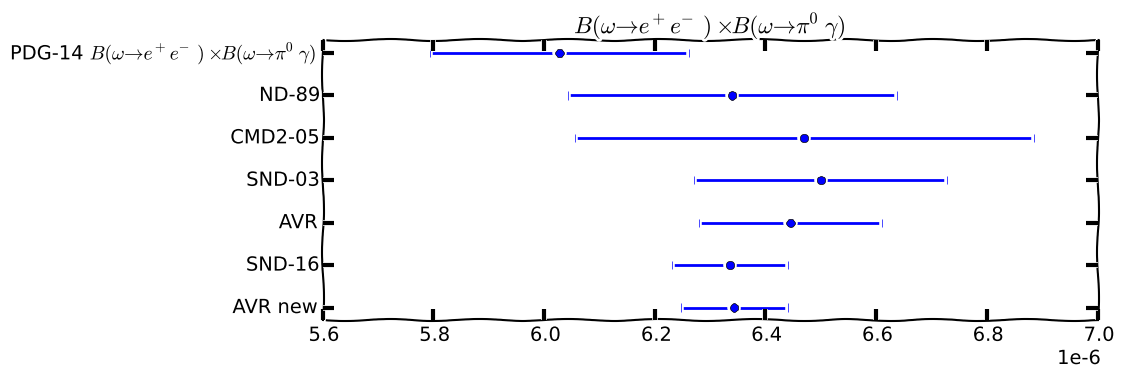
\includegraphics[width=.85\textwidth]{{img/Bw2ee_x_Bwpi0g}.png}
    \caption{$B(\omega \to e^+e^-) \times B(\omega \to \pi^0\gamma)$.
    PDG-14 --- \cite{Agashe:2014kda},
    ND-89 --- \cite{Dolinsky:1988zy},
    CMD2-05 --- \cite{Akhmetshin:2004gw},
    SND-03 --- \cite{Achasov:2003ed},
    AVR --- среднее \cite{Dolinsky:1988zy, Akhmetshin:2004gw, Achasov:2003ed},
    SND-16 --- \cite{Achasov:2016bfr},
    AVR new --- среднее \cite{Dolinsky:1988zy, Akhmetshin:2004gw, Achasov:2016bfr}}
    \label{fig:BweeXBwpig}
\end{figure}
Эта разница вызвана существованием противоречием между измереными значениями
$B( \omega \to \pi^0 \gamma ) \times B(\omega \to e^+ e^-)$,
$B( \omega \to \pi^0 \gamma ) \times B (\omega \to \pi^+ \pi^- \pi^0)$ и
$B( \omega \to \pi^0 \gamma ) / B (\omega \to \pi^+ \pi^- \pi^0)$ (см. Рис.~\ref{fig:Gw2pi0g_o_Gw2pippimpi0}).
Два последних выражения известны с точностью \SI{1.6}{\percent} и \SI{1.8}{\percent} соответственно,
и определяют нынешнее значение $B( \omega \to \pi^0 \gamma )$,
приводимое ПДГ.
Для прояснения этого противоречия необходимо улучшение точности
измерения сечения $e^+e^- \to \pi^0\gamma$ в области $\omega$-резонанса.

\begin{figure}[htbp]
    \centering
    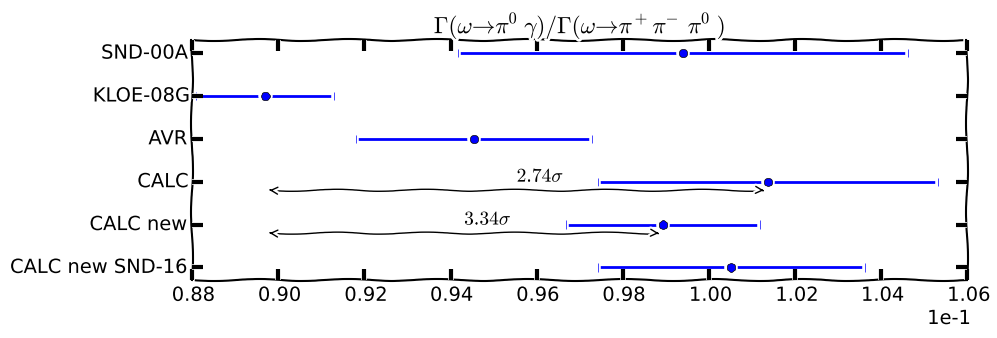
\includegraphics[width=.85\textwidth]{{img/Gw2pi0g_o_Gw2pippimpi0}.png}
    \caption{Отношение ширины распада $\omega \to \pi^0 \gamma$ к $\Gamma (\omega \to \pi^+ \pi^- \pi^0)$.
    SND-00A --- \cite{Aulchenko:2000zq},
    KLOE-08G --- \cite{Ambrosino:2008gb},
    AVR --- средние значение предыдущих двух,
    CALC --- среднее \cite{Akhmetshin:2004gw, Achasov:2003ed, Dolinsky:1988zy} делённое на среднее \cite{Akhmetshin:2003zn, Aubert:2004kj, Achasov:2003ir},
    CALC new --- среднее \cite{Akhmetshin:2004gw, Achasov:2016bfr, Dolinsky:1988zy} делённое на среднее \cite{Akhmetshin:2003zn, Aubert:2004kj, Achasov:2003ir},
    CALC new SND-16 --- \cite{Achasov:2016bfr} делённое на среднее \cite{Akhmetshin:2003zn, Aubert:2004kj, Achasov:2003ir}}
    \label{fig:Gw2pi0g_o_Gw2pippimpi0}
\end{figure}

\subsubsection{\texorpdfstring{$\rho \to \pi^0 \gamma$}{rho --> pi0 gamma}}
\label{rho-to-pi0-gamma}

Точность измерения относительной вероятности распада
$\rho \to \pi^0 \gamma$ составляет \SI{13}{\percent} и определяется статистикой
существующих измерений.

\subsubsection{\texorpdfstring{$\phi \to \pi^0 \gamma$}{}}
\label{phi-to-pi0-gamma}

Формальная точность значения ПДГ вероятности распада
$\phi \to \pi^0 \gamma$ лучше \SI{5}{\percent}.
Оно получено путём усреднения измерений \cite{Achasov:2000zd,Akhmetshin:2004gw} с систематической
ошибкой порядка \SI{8}{\percent} каждое.
Систематическая ошибка возникает из
неопределённости интерференции нерезонансной амплитуды с амплитудой
$\phi \to \pi^0 \gamma$ распада. Нерезонансная амплитуда определяется
вкладами хвостов резонансов $\omega$ и $\rho^0$, заодно дают вклад и
высшие возбуждения векторных мезонов.

Чтобы уменьшить неопределённость таких вкладов, необходимо улучшить
точность измерения сечения $e^+e^- \to \pi^0 \gamma$ в широком диапазоне
энергий от энергий \SI{\sim 300}{\MeVr} до \SI{2}{\GeVr}.

\subsection{Аномальный магнитный момент мюона}\label{mu-amm}

Как люди не могут забыть Герострата, сжёгшего храм Артемиды, так и физики
элементарных частиц рвутся попасть в истории кардинально изменив или
изничтожив современную парадигму науки --- Стандартную Модель. Некоторые
из них ищут Новую Физику пробуя другие области энергии и массы, кто-то
ищет новые распады, другие же могут мерить что-то очень точно и
сравнивать это с предсказаниями теории.
К последней группе относится изучение аномального магнитного момента мюона.

%%%%%%%%%%%%%%%%%%%%%%%%%%%%%%%%%%%%%%%%%%%%%%%%%%%%%%%%%%%%%%%%%%%%%%%%%%%%%%%%
\subsubsection{История}\label{g-2-history}

Экспериментальные измерения $a_\mu$ впервые было осуществлено в СЛАКе \cite{Garwin:1960zz}.
Затем последовала серия измерений в ЦЕРНе, уступившее свое место эксперементу в БНЛ.
В настоящий момент готовится два эксперимента по измерению $g_\mu-2$: в ФНАЛ \cite{Grange:2015fou} и Джей-ПАРКе \cite{Saito:2012zz}.


%%%%%%%%%%%%%%%%%%%%%%%%%%%%%%%%%%%%%%%%%%%%%%%%%%%%%%%%%%%%%%%%%%%%%%%%%%%%%%%%
\subsubsection{Вклады в \texorpdfstring{$g_\mu-2$}{muon g-2}}
\label{contribution-to-g-2}

Предсказываемый в рамках СМ аномальный магнитный момент мюона $f_\mu^{\text{SM}}$ принято представлять суммой трёх слагаемых
\begin{equation}
    a_\mu^{\text{SM}} = a_\mu^{\text{QED}} + a_\mu^{\text{EW}} + a_\mu^{\text{had}},
\end{equation}
где $a_\mu^{\text{QED}}$ --- электродинамический вклад,
$a_\mu^{\text{EW}}$ --- вклад слабых взаимодействий,
$a_\mu^{\text{had}}$ --- вклад сильных взаимодействий.

Не сомтре на то, что вклад $a_\mu^{\text{had}}$ меньше $a_\mu^{\text{QED}}$ примерно на четыре порядка,
его значение примерно в 100 раз превышает точность последного эксперимента в БНЛ.
Последние обстоятельство вместе с планируемым улучшением измерения $a_\mu$ в четыре раза
требует вычисления $a_\mu^{\text{had}}$ с относительной точностью \SIrange{1}{0.1}{\percent}.

\begin{figure}[htbp]
    \begin{minipage}[t]{0.24\textwidth}
        \centering
        \begin{tikzpicture}
        \begin{feynman}
			\vertex (a);
			\vertex [below = 1cm of a] (b);
			\vertex [below left = 18.8562mm of b] (c1);
			\vertex [below right = 18.8562mm of b] (c2);
			\vertex [below left = 28.2843mm of b] (d1);
			\vertex [below right = 28.2843mm of b] (d2);
			\vertex [below right = 0mm of d1] {$\mu$};
			\vertex [below left = 0mm of d2] {$\mu$};
			% \node [below = of d1] {$\mu$};
			\vertex [right = 9.3333mm of c1, blob] (c3) {};
			% \vertex [right = 8mm of c3] (c4);
			\vertex [below right = 0mm of a] {$\gamma$};
		    
		    \diagram* [small] {
			    (a) -- [photon] (b),
			    (d1) -- [fermion] (c1) -- [fermion] (b) -- [fermion] (c2) -- [fermion] (d2),
		    	(c1) -- [photon] (c3) -- [photon] (c2),
		    	% (c4) -- [photon] (c2),
		 	};
		\end{feynman}
		\end{tikzpicture}
        \caption{Ведущий адронный вклад в $a_\mu$.}\label{diag:hvp}
    \end{minipage}
    \hfill
    \begin{minipage}[t]{0.24\textwidth}
        \centering
        \begin{tikzpicture}
		\begin{feynman}
			\vertex (a);
			\vertex [below = 1cm of a] (b);
			\vertex [below left = 18.8562mm of b] (c1);
			\vertex [below right = 18.8562mm of b] (c2);
			\vertex [below left = 28.2843mm of b] (d1);
			\vertex [below right = 28.2843mm of b] (d2);
			\vertex [right = 7.3333mm of c1, dot, blue] (c3) {};
			\vertex [right = 12mm of c3, dot, blue] (c4) {};
			\vertex [below right = 0mm of d1] {$\mu$};
			\vertex [below left = 0mm of d2] {$\mu$};
			\vertex [below right = 0mm of a] {$\gamma$};
		    
		    \diagram* [small] {
			    (a) -- [photon] (b),
			    (d1) -- [fermion] (c1) -- [fermion] (b) -- [fermion] (c2) -- [fermion] (d2),
		    	(c1) -- [photon] (c3),
		    	(c4) -- [photon] (c2),
		    	(c3) -- [photon, half left] (c4) -- [scalar, blue, very thick, half left, edge label={\(\pi^{0}\), \(\eta\)}] (c3),
		 	};
		\end{feynman}
		\end{tikzpicture}
        \caption{Ведущий адронный вклад в $a_\mu$ связанный с $e^+ e^- \to ( \pi^0, \, \eta ) \gamma$.}\label{diag:hvp_Pg}
    \end{minipage}
    \hfill
    \begin{minipage}[t]{0.24\textwidth}
        \centering
        \begin{tikzpicture}
		\begin{feynman}
			\vertex (a);
			\vertex [below = 7mm of a, blob] (a1) {};
			\vertex [below = 1cm of a] (b);
			% \vertex [below = 7mm of a, blob] (a1) {};
			\vertex [below left = 17.2132mm of b] (c1);
			\vertex [below left = 4mm of b] (b1);
			\vertex [below = 4mm of b] (b2);
			\vertex [below right = 4mm of b] (b3);
			% \vertex [below = 11mm of b] (c2);
			% \vertex [right = 15mm of c1] (c2);
			\vertex [below = 12mm of b] (c2);
			\vertex [below right = 17.2132mm of b] (c3);
			\vertex [below left = 7.0711mm of c1] (d1);
			\vertex [below right = 7.0711mm of c3] (d2);
			\vertex [below right = 0mm of d1] {$\mu$};
			\vertex [below left = 0mm of d2] {$\mu$};
			\vertex [below right = 0mm of a] {$\gamma$};
		    
		    \diagram* [small] {
			    (a) -- [photon] (a1),
			    (b1) -- [photon] (c1),
			    (b3) -- [photon] (c3),
			    (d1) -- [fermion] (c1) -- [fermion] (c2) -- [fermion] (c3) -- [fermion] (d2),
			    (b2) -- [photon] (c2),
		 	};
		\end{feynman}
		\end{tikzpicture}
        \caption{Ведущий адронный вклад света на свете в $a_\mu$.}\label{diag:lbl}
    \end{minipage}
    \hfill
    \begin{minipage}[t]{0.24\textwidth}
        \centering
        \begin{tikzpicture}
		\begin{feynman}
			\vertex (a);
			\vertex [below = 1cm of a, dot, blue] (b) {};
			\vertex [below left = 10.6066mm of b, dot, blue] (c) {};
			\vertex [below left = 10.6066mm of c] (d1);
			\vertex [right = 15mm of d1] (d2);
			\vertex [below right = 21.2132mm of b] (d3);
			\vertex [below left = 28.2843mm of b] (e1);
			\vertex [below right = 28.2843mm of b] (e2);
			\vertex [below right = 0mm of e1] {$\mu$};
			\vertex [below left = 0mm of e2] {$\mu$};
			\vertex [below right = 0mm of a] {$\gamma$};
					    
		    \diagram* [small] {
			    (a) -- [photon] (b),
			    (b) -- [scalar, very thick, blue, edge label'={\(\pi^{0}\), \(\eta\)}] (c),
			    (c) -- [photon] (d1),
			    (c) -- [photon] (d2),
			    (b) -- [photon] (d3),
			    (e1) -- [fermion] (d1) -- [fermion] (d2) -- [fermion] (d3) -- [fermion] (e2),
		 	};
		\end{feynman}
		\end{tikzpicture}
        \caption{Ведущий адронный вклад света на свете в $a_\mu$ связанный с $e^+ e^- \to ( \pi^0, \, \eta ) \gamma$.}\label{diag:lbl_Pg}
    \end{minipage}
\end{figure}
В свою очередь во вкладе сильных взаимодействий принято выделять три слагаемых:
рассеяние света на свете $a_\mu^{\text{had, LbL}}$ (диаграмма~\ref{diag:lbl}),
вклады первого $a_\mu^{\text{had, LO}}$ (диаграмма~\ref{diag:hvp}) и второго $a_\mu^{\text{had, NLO}}$ порядков:
\begin{equation}
    a_\mu^{\text{had}}
    =
    a_\mu^{\text{had, LO}}
    +
    a_\mu^{\text{had, NLO}}
    +
    a_\mu^{\text{had, LbL}}.
\end{equation}

В то время как вычисление вкладов $a_\mu^{\text{QED}}$ и $a_\mu^{\text{EW}}$ успешно происходит с использованием теории возмущений ввиду малости соответствующих констант связи,
вклад сильных взаимодействий трубует иного подхода в области характерных передач импульса меньше \SI{2}{\GeVr}.
Ведущий вклад $a_\mu^{\text{had, LO}}$ рассчитывается и использованием дисперсионного соотношения
\cite{Bouchiat1961, Durand:1962zzb, Kinoshita:1967txv, Gourdin:1969dm},
позволяющего использовать экспериментальные данные \cite{Jegerlehner:2017gek}.
\begin{equation}
   	a_\mu^{\text{had}} =
   	\left( \frac{\alpha m_\mu}{3 \pi} \right)^2
   	\left(
   		\int_{{m_{\pi^0}}^2}^{{E_{\text{cut}}}^2} \dif s
   		\frac{ R_{\text{had}}^{\text{data}}(s) \hat{K}(s) }{ s^2 }
   		+
   		\int_{{E_{\text{cut}}}^2}^{\infty} \dif s
   		\frac{ R_{\text{had}}^{\text{pQCD}}(s) \hat{K}(s) }{ s^2 }
   	\right) ,
\end{equation}
где
$ m_\mu $ --- масса мюона;
$ m_{\pi^0}$ --- масса нейтрального пиона;
$ E_{\text{cut}} $ --- энергия перехода от использование вычислений на основе экспериментальных данных к результатам полученным в рамках пертрубативной КХД;
интегрирование идёт по квадрату энергии системы $s$;
$ R_{\text{had}}^{\text{data}}(s) $ и $ R_{\text{had}}^{\text{pQCD}}(s) $ --- $R$-отношение вычисленное по экспериментальным данным и согласно КХД, соответственно:
\begin{equation}
	R_{\text{had}} (s) =
   	\sigma(e^+ e^- \to \text{hadrons})
  	/
  	\frac{4 \pi \alpha(s)}{3 s} .
\end{equation}
Ядро интегрирования $\hat{K}(s)$ определено следующим образом
\begin{equation}
	\hat{K}
  	=
   	\frac{3 s}{{m_\mu}^2}
  	\int_0^1 \dif x
  	\frac{ x^2 (1-x) }{ x^2 + \frac{s}{{m_\mu}^2} (1-x) } .
\end{equation}

Таким образом,
вклад изучаемых процессов в лидирующий влад адронной поляризации вакуума можно представить диаграммой~\ref{diag:hvp_Pg}.

Расчёт вклада света на свете представляет наибольшую сложность,
так как он не поддаётся вычислениям ни в рамках теории возмущений КХД,
ни связыванию с экспериментальными данными использую дисперсионное соотношение.
Производимые расчёты оказываются модельно зависимы,
приводя к сравнительно большой неопределённости вычислений.
Адронный блок диаграммы~\ref{diag:lbl} представляется в виде обемена адронами.
Доминирующий вклад вносят псевдоскалярные мезоны $\pi^0$, $\eta$, $\eta^\prime$,
при этом процесс выгляит как на диаграмме~\ref{diag:lbl_Pg}.
Развитие моделей,
фиксирование их свободных параметров и проверка,
разумеется связано с использованием экспериментальных данных.
Косательно псевдоскалярных мезонов $P$ особенно ценными является измерение форм-фактора
$F_P ( {q_1}^2, \, {q_2}^2 )$.
Однако, полезными также являются и вся остальная достпуная информация,
в том числе сечение реакция типа $e^+ e^- \to P \gamma$.


%%%%%%%%%%%%%%%%%%%%%%%%%%%%%%%%%%%%%%%%%%%%%%%%%%%%%%%%%%%%%%%%%%%%%%%%%%%%%%%%
\subsubsection{Расчёт вкладов в различных моделях}
\label{contribution-calculation}


Как было сказано выше,
невозможность прямого вычисления $a_\mu^{\text{had, LO}}$
в теории сильных взаимодействий обойдена при помощи дисперсионно соотношения,
требущего в свою очередь знания зависимости сечений процессов
$e^+ e^- \to \gamma^* \to \text{hadrons}$
от энергии в системе центра масс $\sqrt{s}$.
Последнее важно как для инклюзивного,
так и для эксклюзивного вычисления $R_{\text{had}}^{\text{data}}$.
В виду того,
что экспериметальные данные доступны в конретных точках или диапазонах по энергии,
и иногда могут и отсутсвовать вовсе или их точность неудовлетворительна,
а в то же время для других каналов и энергий наблюдается перекрытие,
требуется производить аппроксимацию или усреднение.
Ниже будет упомянуто о различных методиках решения задачи вычисления $R_{\text{had}}^{\text{data}}$,
приминительно к вкладам процессов $\pi^0 \gamma$ и $\eta \gamma$.


%%%%%%%%%%%%%%%%%%%%%%%%%%%%%%%%%%%%%%%%%%%%%%%%%%%%%%%%%%%%%%%%%%%%%%%%%%%%%%%%
% KNT18
В статье \cite{KNT18} экспериментальные данные разбиваются на кластеры.
Внутри кластера идёт поиск центра тяжести и его ошибки путём иттерационной минимизации $\chi^2$ сечения
представленного ломанной кривой, соединяющий центры кластеров.
Таким образом дальнейшее интгрирование в том же линейном приближении является оптимпальным вариантом вычисления вкладов в $a_\mu^{\text{had, LO}}$.
Полученные результаты касательно процессов $\pi^0 \gamma$ и $\eta \gamma$ приведены в таблицах~\ref{tab:amm_pi0g}, \ref{tab:amm_etag}.
%%%%%%%%%%%%%%%%%%%%%%%%%%%%%%%%%%%%%%%%%%%%%%%%%%%%%%%%%%%%%%%%%%%%%%%%%%%%%%%%

\begin{table}
	\centering
	\caption{Вклад в $a_\mu^{\text{had, LO}}$ и $\Delta \alpha_{\text{had}} ({M_Z}^2) $ процесса 
		$e^+ e^- \to \pi^0 \gamma$.}\label{tab:amm_pi0g}
	\begin{tabular}{ccccc}
		Энергия, \si{\GeVr} & $a_\mu^{\text{had, LO}}$ & $\Delta \alpha_{\text{had}} ({M_Z}^2) $ & Источник \\
		\hline
		$[m_\pi , \, 0.6]$ & \num{0.12 \pm 0.01} & \num{0.00 \pm 0.00} & \cite{KNT18} \\
		$[0.6 , \, 1.350]$ & \num{4.46 \pm 0.10} & \num{0.36 \pm 0.01} & \cite{KNT18} \\
		$[m_\pi , \, 1.8]$ & $4.29 \pm 0.06 \pm 0.04 \pm 0.07$ & $0.35 \pm 0.00 \pm 0.00 \pm 0.01$ & \cite{Davier:2017zfy} \\
		$[0.318 , \, 2]$ & \num{4.06 \pm 0.16} & \num{0.35 \pm 0.01} & \cite{Jegerlehner:2017gek} \\
		$[m_\pi , \, 0.6]$ & \num{0.13 \pm 0.01} &  & \cite{Ahmadov:2010hq} \\
		$[0.6 , \, 1.03]$ & \num{4.5 \pm 0.15} &  & \cite{Ahmadov:2010hq}
	\end{tabular}
\end{table}

\begin{table}
	\centering
	\caption{Вклад в $a_\mu^{\text{had, LO}}$ и $\Delta \alpha_{\text{had}} ({M_Z}^2) $ процесса 
		$e^+ e^- \to \eta \gamma$.}\label{tab:amm_etag}
	\begin{tabular}{cccc}
		Энергия, \si{\GeVr} & $a_\mu^{\text{had, LO}}$ & $\Delta \alpha_{\text{had}} ({M_Z}^2) $ & Источник \\
		\hline
		$[m_\eta , \, 0.66]$ & \num{0.12 \pm 0.01} & \num{0.00 \pm 0.00} & \cite{KNT18} \\
		$[0.66 , \, 1.35]$ & \num{4.46 \pm 0.10} & \num{0.36 \pm 0.01} & \cite{KNT18} \\
		$[m_\eta , \, 1.8]$ & $0.65 \pm 0.02 \pm 0.01 \pm 0.01$ & $0.08 \pm 0.00 \pm 0.00 \pm 0.00$ & \cite{Davier:2017zfy} \\
		$[0.318 , \, 2]$ & \num{0.56 \pm 0.02} & \num{0.06 \pm 0.00} & \cite{Jegerlehner:2017gek} \\
		$[0.69 , \, 1.33]$ & \num{0.73 \pm 0.03} &  & \cite{Ahmadov:2010hq}
	\end{tabular}
\end{table}

%%%%%%%%%%%%%%%%%%%%%%%%%%%%%%%%%%%%%%%%%%%%%%%%%%%%%%%%%%%%%%%%%%%%%%%%%%%%%%%%
% DHMZ17
Авторы работы \cite{Davier:2017zfy} для вычисления вкладов проводят квадратичную интерполяцию экспериментальных данных для каждого канала каждого анализа.
Полученное приблежение используют для вычисления сечений в бинах шириной \SI{1}{\MeVr}.
Далее в каждом бине каждого канала идёт усреднение по всем измерением.
В случае противоречивости данных ошибка их комбинации масштабируется.
%%%%%%%%%%%%%%%%%%%%%%%%%%%%%%%%%%%%%%%%%%%%%%%%%%%%%%%%%%%%%%%%%%%%%%%%%%%%%%%%

%%%%%%%%%%%%%%%%%%%%%%%%%%%%%%%%%%%%%%%%%%%%%%%%%%%%%%%%%%%%%%%%%%%%%%%%%%%%%%%%
% FJ17
% BDDJ12&17
В работах \cite{Benayoun:2016krn, Jegerlehner:2017gek}
расчёт вкладов в АПВ идёт на основе комбинации модели доминантности векторных мезонов
с моделью нарушения скрытой локальной симметрии.
Полученной комбинацией идёт подгонка экспериментальных данных сразу в нескольких каналах $e^+ e^-$-аннигиляции
и спектральных функций $\tau$-лептона.
%%%%%%%%%%%%%%%%%%%%%%%%%%%%%%%%%%%%%%%%%%%%%%%%%%%%%%%%%%%%%%%%%%%%%%%%%%%%%%%%

%%%%%%%%%%%%%%%%%%%%%%%%%%%%%%%%%%%%%%%%%%%%%%%%%%%%%%%%%%%%%%%%%%%%%%%%%%%%%%%%
% AKV10
В статье \cite{Ahmadov:2010hq}
используется расширенная модель Намбу--Иона-Лазинио,
для определения параметров которой происходит подгонка экспериментальных данных,
а затем вычисление вкладов в $a_\mu^{\text{had, LO}}$.
%%%%%%%%%%%%%%%%%%%%%%%%%%%%%%%%%%%%%%%%%%%%%%%%%%%%%%%%%%%%%%%%%%%%%%%%%%%%%%%%



\subsection{Структура мезонов}
\label{meson-structures}

Являясь частью СМ квантовая хромодинамика отвечает за процессы с участием адронов. Однако, она весьма ограничена в использовании для области энергий с характерной передачей импульса ниже \SI{1}{\GeVr}.
Это привело к популярности феноменологических подходов к описанию физики в данной области энергий.
Используемые модели обладают рядом свободных параметров,
которые можно фиксировать из экспериментальных данных.
С другой стороны,
такие модели не только подгоняют уже имеющиеся данные,
но обладают предсказательной силой,
величину которой хорошо бы проверять не только качественно,
но и числено.
Для двух этих целей --- определение свободных параметров и проверка верности ---
прекрасно подходят сечения изучаемых процессов.
Оба они относятся к магнитным радиационным переходам М1,
что делает их хорошим инструментом для изучения структуры мезонов в свете различных феноменологических моделей,
например кварковой модели с $SU(3)$ или даже с $SU(6)$ симметрией.

\resizebox{.3\paperwidth}{!}{%
\begin{tikzpicture}
	\begin{feynman}
		%\vertex (a) {\(e^{-}\)};
		%\vertex [below right=of a] (b);
		%\vertex [below left=of b] (c) {\(e^{+}\)};
		\vertex (b);
		\vertex [above left=of b] (a) {\(e^{-}\)};
		\vertex [below left=of b] (c) {\(e^{+}\)};
		\vertex [right=of b, dot, blue] (d) {};
		\vertex [above right=of d] (f1) {\(\gamma\)};
	    \vertex [below right=of d, dot, blue] (m1) {};
	    \vertex [above right=of m1] (f2) {\(\gamma\)};
	    \vertex [below right=of m1] (f3) {\(\gamma\)};
		    
	    \diagram* [small] {
		    (a) -- [fermion] (b) -- [fermion] (c),
		    (b) -- [photon, edge label=\(\gamma^{*}\)] (d) [blob],
		    (d) -- [photon] (f1),
		    (d) -- [scalar, blue, very thick, edge label'={\(\pi^{0}\), \(\eta\), (\(\eta^\prime\))}] (m1),
		    (f3) -- [photon] (m1) [blob] -- [photon] (f2),
			% (m1) -- [photon] (f3),
	 	};
	\end{feynman}
\end{tikzpicture}
}

Особый интерес представляют структуры мезонов $\eta$ и $\eta^\prime$, так как в них допускается наличия вкладов $c\bar{c}$-кварков или примесь глюонов. 

В своей статье О'Доннелл \cite{ODonnell:1981sj} исследует кварковый состав мезонов в
рамках кварковой модели и проверяет получаемые результаты с помощью
экспериментальных данных, в то числе, по магнитнодипольным переходам
векторных мезонов в пару фотон-псевдоскаляр.

%В статье Болла, Фрере, Титгэт \cite{Ball:1995zv} ках феноменологической модели.% что за модель?
%С этой целью рассматриваются радиационные распады
%$P \to \gamma \gamma$, $V \to P \gamma$ и $P \to V \gamma$. Упор
%делается на работу с основными состояниями, таким образом не учитываются
%вклады возбуждённых состояний лёгких векторных мезонов.

Эскрибано и Надаль \cite{Escribano:2007cd} исследовали вклад в глюонов в состояния $\eta$
и $\eta(958)$ провядя феноменологический анализ радиационных распадов
$V (P) \to P (V) \gamma$ в рамках нарушенной SU(3) с учётом
пространственного перекрытия волновых функций $| V \rangle$ и
$|P \rangle$. Авторы заключают, что глюонная составляющая в $\eta$ и
$\eta(958)$ пренебрежимо мала, угол смешивание
$\eta-\eta^\prime = \ang{41.4 \pm 1.3}$, и подчёркивают важность
экспериментальных данных по $(\rho, \, \omega, \, \phi ) \to \eta \gamma$ для
проведённых вычислений.

В статье Бенаёун, ДельБуоно, Эйдельмана, Иванченко и О'Коннелла \cite{Benayoun:1999fv} даётся разбор
вопроса о совместном согласованном описании радиационных и лептонных
распадов лёгких мезонов ($V(P) \to P(V)\gamma$, $P \to \gamma \gamma$ и
$V \to e^+ e^-$).


\subsection{Другие измерения}\label{other-measurments}

Данные измерения не будут являться первыми, однако,
они возможно смогут претендовать на сравнимые или улучшенные точности в уже исследованных областях энергии $\sqrt{s}$
или быть даже первыми и одними из первых в других.
Ниже приведены данные о предыдущих измерениях с целью выявления современной ситуации в этой области извлечения данных природы.
Наиболее значимые результаты измерений приведены на рисунке~\ref{fig:cs_pi0g_prev} для процесса $e^+ e^- \to \pi^0 \gamma$
и на рисунке~\ref{fig:cs_etag_prev} для $e^+ e^- \to \eta \gamma$.

\begin{figure}[htbp]
	\begin{minipage}[T]{.48\textwidth}
		\centering
		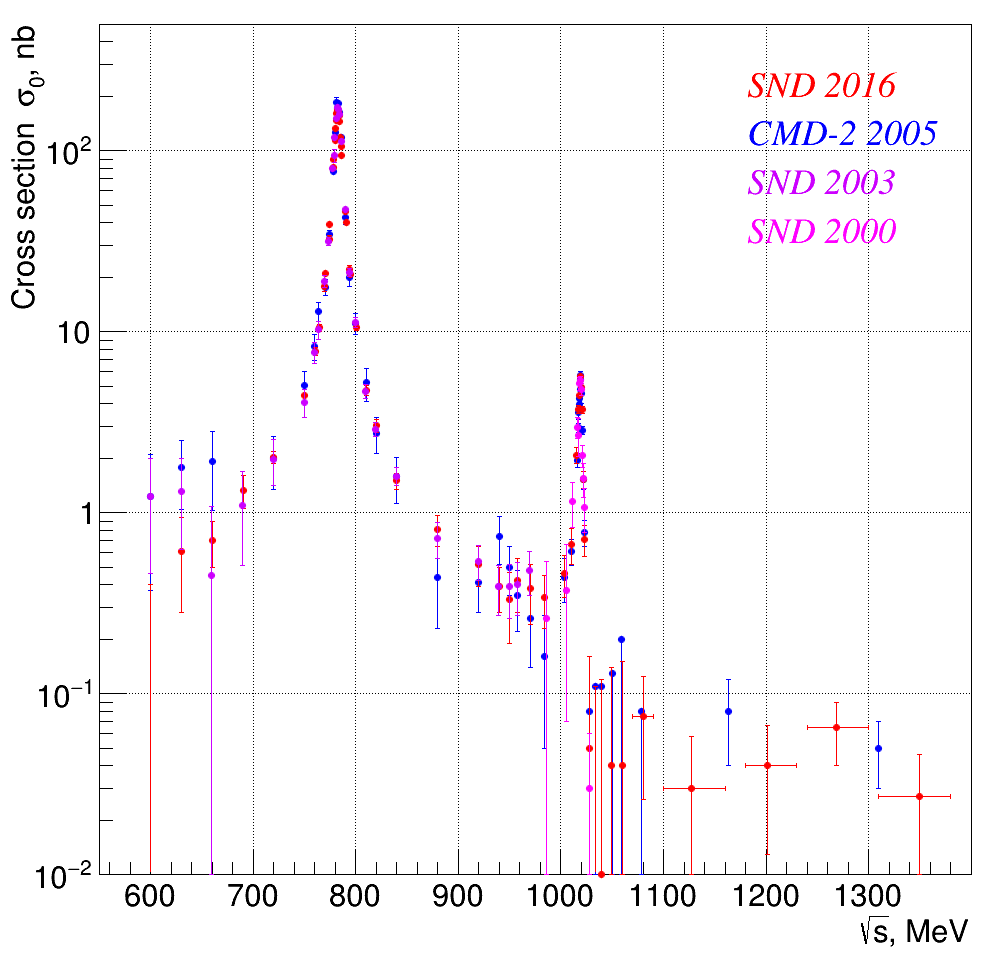
\includegraphics[width=\textwidth]{img/cs_pi0g_550_1400.png}
		\caption{Некоторые предыдущие измерения сечения $e^+ e^- \to \pi^0 \gamma$.}\label{fig:cs_pi0g_prev}
	\end{minipage}
	\hfill
	\begin{minipage}[T]{.48\textwidth}
		\centering
		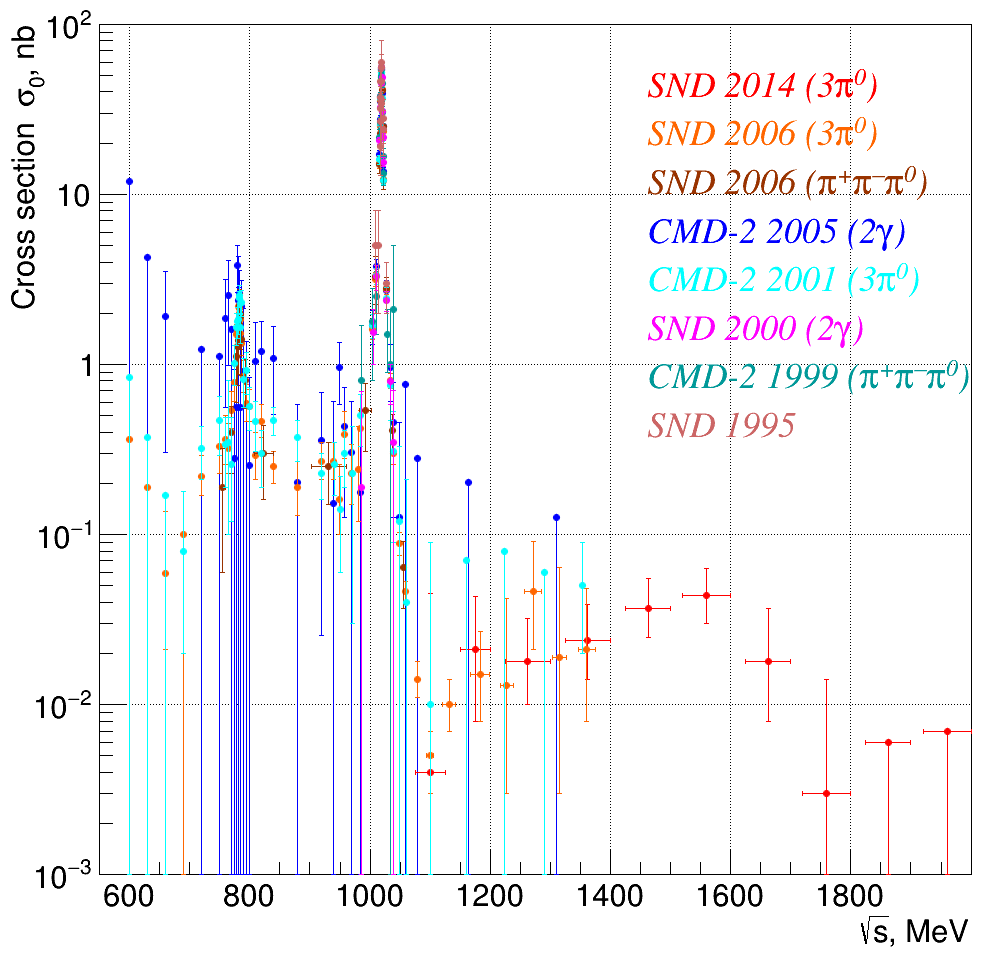
\includegraphics[width=\textwidth]{img/cs_etag_550_2000.png}
		\caption{Некоторые предыдущие измерения сечения $e^+ e^- \to \eta \gamma$.}\label{fig:cs_etag_prev}
	\end{minipage}
\end{figure}

Сечение процесса $e^+e^-\to\eta\gamma$ исследовалось во многих экспериментах.
Первые опубликованные данные появились в 1976 году из Орсая \cite{Cosme:1975rs}.
Дальнейший поток данных в основном происходит из установок Новосибирска, начиная с работы выполненной на детекторе НД \cite{Druzhinin:1984zq} и продолжая данными с КМД-2 \cite{Akhmetshin:1995vz, Akhmetshin:1999zv, Akhmetshin:2001hm, Akhmetshin:2004gw} и СНД \cite{Achasov:1997nq, Achasov:2000zd, Achasov:2006dv, Achasov:2013eli}.
Также известно измерение сечения реакции на детекторе BaBar \cite{Aubert:2006cy}.

Сечение процесса $e^+e^-\to\pi^0\gamma$ измерено несколько раз, начиная с работы в Орсаи \cite{Cosme:1975rs} и продолжая работами в Новосибирске \cite{Druzhinin:1984zq, Achasov:2000zd, Achasov:2003ed, Akhmetshin:2004gw, Achasov:2016bfr}.



\subsection{Отбор событий}

Отбор разбивается на несколько шагов. В начале пути отбираются полностью нейтральные события с тремя и более фотонами.
Причём от каждого фотона требуется, чтобы его энергия была больше \SI{30}{\MeVr} и полярный угол не тяготеет к вакуумной трубе.
Для таких событий вычисляется полная энергия $E_{\text{tot}}$ и импульс $P_{\text{tot}}$ системы частиц.
Характерное распределение представлено на рисунке~\ref{fig:EtvsPt5095}.
Сгущение событий около точки $P_{\text{tot}} = \SI{0}{\MeVr}$ и $E_{\text{tot}} = \sqrt{s}$ отвечаем искомым событием.
От этой группы тянется два хвоста под углами \ang{45} вверх и вниз.
Равное отколонение импульса $|P_{\text{tot}} - \SI{0}{\MeVr}|$ и энергии $|E_{\text{tot}} - \sqrt{s}|$
---
указание на то,
что данная девиация вызвана одной частицей.
Хвост уходящий вверх соответствует учёту излишней энергии в системе,
как правило такое соответствует тому,
что фотонным кластерам приписывается излишнее энерговыделение или имеется дополнительный кластер не возникший в следствие $e^+e^-$-аннигиляции,
к которой относится конкретное событие.
Хвост уходящий вниз, наоборот свидетельствует о недостатке энергии-импульса в системе.

\begin{figure}
	\centering
	\label{fig:EtvsPt5095}
	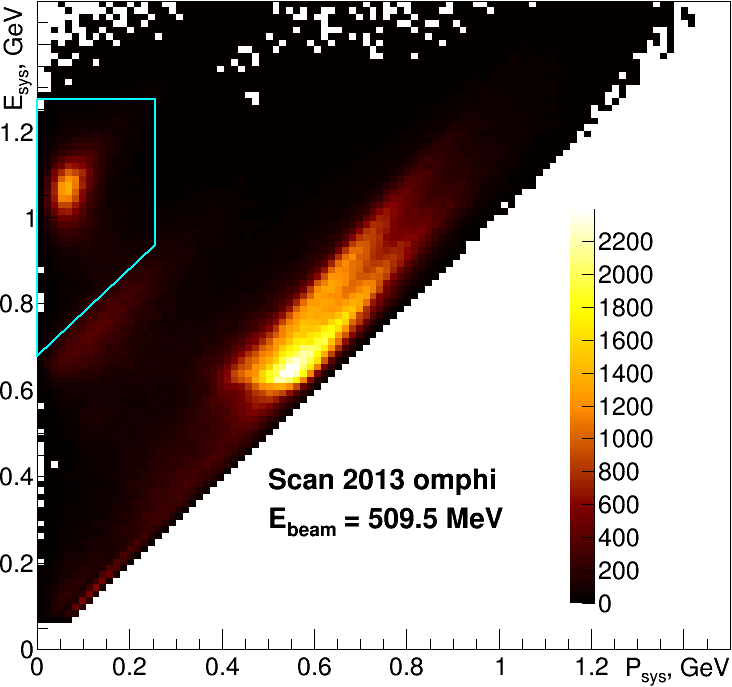
\includegraphics[width=.5\textwidth]{img/EtvsPt5095.png}
	\caption{Зависимость полной энергии события $E_{\text{tot}}$ от модуля полного импульса $P_{\text{tot}}$.
		Данные эксперимета, сезон 2013 $\omega \ \phi$, $E_{\text{beam}} = \SI{509.5}{\MeVr}$.
		Циановой линией обозначены условия отбора.}
\end{figure}

Теперь наступает шаг по отбору событий, в которых импульс системы близок к нулю,
а энергии к удвоенной энергии пучков.
Такой отбор направлен на те события,
где детектор зарегистрировал все частицы конечного состояния,
в то время как дополнительные кластеры в калориметре не дают значительного вклада.

На следующим шаге проводится кинематическая реконструкция событий.
В неё заложены законы сохранения энергии-импульса системы в целом и общая точка вылета фотонов.
Наличие промежуточных состояний $\pi^0$ или $\eta$ не требуется,
так как это оставляет крайне мало параметров последующей селекции сигнальных событий от фотона.
Если в событие присутствует более трёх фотонов,
то кинематическая реконструкция проводится для каждой возможной тройки и оставляется та,
что имеет наименьший $\chi^2$.
Подробнее о процедуре кинематической реконструкции изложено в разделе~\ref{sec:kf}.

Теперь, 
когда составлен набор трёхчастичных событий, 
отбрасываются все события, 
в которых не один из фотонов не полетел в центральную часть калориметра, 
а именно в систему \ce{LXe}. 
Такое условие предполагает наличие точки конверсии фотона,
определённой по полосковой электронике \ce{LXe} с хорошим координатным разрешением.

На этом отбор кандидатов закончен. 
В дальнейшем они разделяются на две большие пересекающиеся подгруппы: 
хотя бы один фотон попал в \ce{LXe} и все фотоны попали в центральную часть калориметра.
Попадание в центральную часть определяется по полярному углу фотона до кинематической реконструкции как $0.9 < \theta < \pi - 0.9$.



\subsubsection{Кинематическая реконструкция}
\label{sec:kf}

В ходе физической реконструкции событий закладывается гипотеза о знании точки вылета фотонов.
Предполагая угол влёта фотона в калориметр,
реконструируется его энергия по зарегистрированному энерговыделению.
Для нейтральных событий точка взаимодействия начальных лептонов не определена вдоль их движения и,
как следствие,
делается предположение о их вылете из центральной плоскости детектора $z = 0$.
Естественно,
это ухудшает разрешение параметров фотонов.
С целью преодоления такого недостатка проводится кинематическая реконструкция событий,
приводящая к улучшению ситуации,
что особенно ярко проявляется на распределениях инвариантных масс фотонов,
отвечающих мезонам.

Алгоритм кинематической реконструкции был разработан на основе работ \cite{Bukin2003-27, Bukin2005-51, Bukin2008-3}.
В них были описаны несколько подходов к составлению и минимизации функционалов.
Выбор остановился на составлении функционала со штрафными функциями,
сила которых регулируется весовыми коэффициентами
---
множителями Лагранжа.
Саму минимизацию было решено проводить численным методом.

В основу кинематической реконструкции заложены законы сохранения энергии-импульса системы в предположении общей точки вылета фотонов.

От энергии фотонов требуется, чтобы их сумма была равна сумме энергий пучков в системе центра масс. Последняя, в лучшем случае измерена с использованием обратного комптоновского рассеяния фотонов лазера на пучке. Следующая по приоритету информации энергии происходит из параметров частиц в различных физических процессах. Наихудший вариант --- уставная энергия ВЭПП-2000. Полный импульс системы полагается равными нулю. Эти два условия в купе говорят об отсутствие рассмотрения радиационного излучения как начальных, так и конечных частиц.
Логичным шагом развития кинематической реконструкции было бы добавления возможности уноса энергии и импульса вдоль оси пучков --- оси $z$.

Общая точка вылета определяется тремя координатами, две из которых фиксированы --- $x$ и $y$ берутся из дерева \textit{tr\_ph} для каждого захода (данный параметры усредняются по всем событиям в заходе с трековыми центральными вершинами в предположении стабильности орбиты пучков).
Разумеется, эти два параметра можно было бы отпустить, но их разрешение несравненно больше, чем у всех остальных, потому это можно отнести к категории мало-играющих факторов в ходе минимизации, разве что они увеличат затраченное время на процесс, и пренебречь ими. 
Третья координата $z$ точки взаимодействия свободна от каких-либо условий, другими словами, её разрешение бесконечно плохое и она не даёт вклада в $\chi^2$.

Когда говорят о координатах фотонов, подразумевается точка конверсии фотона в электрон-позитронную пару, 
являющуюся началом электромагнитного ливня в веществе детектора и не только. 
Определение этой точки конверсии сильно зависит от того, в каком месте она, конверсия, произошла.
Если рассматривать калориметры КМД-3, 
то при рождении ливня в \ce{LXe} в большинстве случаев срабатывает полосковая электроника, позволяя определить координаты с точностью \SIrange[range-phrase=--]{2}{4}{\mm} (?), 
либо по башням, если нет информации с полосок, но точность падает --- глубина равняется половине глубины башни а положение на цилиндрической поверхности средневзвешенному. 
В случае попадания фотона в \ce{BGO} калориметр $r$ и $\varphi$ координаты определяются по центру тяжести энерговыделения, 
а $z$ зависит от угла попадания фотона в калориметр в предположении вылета из центра детектора. 
Когда же фотон зарегистрирован только в \ce{CsI}, то $z$ и $\varphi$ определяются по центру тяжести, 
а $r$ устанавливается равной положению ближайшей к центру грани кристалла.

Координаты конверсии каждого фотона описываются в деревьях \textit{tr\_ph} параметрами $\rho$, $\theta$ и $\varphi$.
К двум последним прилагаются их ошибки $\sigma_\theta$ и $\sigma_\varphi$.
Так как $x_0$ и $y_0$ фиксированы,
то варьирование азимутального угла фотонов корректно.
Однако,
значение полярного угла определяется по точке вылета,
в том числе неопределённой точки $z_0$,
и точке конверсии фотона в калориметре.
Другими словами,
варьирование самого угла $\theta$ двигает две точки.
Поэтому необходимо их развязать для упрощение кинематической реконструкции.
Для цилиндрической части калориметра для варьирование выбирается координата $z$ точки конверсии,
связанная с полярным углом следующим образом:
\begin{equation}
    \theta_i
    =
    \arctg
    \frac{\rho_i}{z_i + \delta z_i + z_0} .
\end{equation}
Для торцевого калориметра варьирование идёт по координате $\rho$,
связь полярного угла с которой определяется как
\begin{equation}
    \theta_i
    =
    \arctg
    \frac{\rho_i + \delta \rho_i}{z_i + z_0} .
\end{equation}

Тем самым минимизация функционала производится варьированием $3 N + 1$ параметром



\begin{equation}
F = w_L L + w_W W + w_N \left( N_1 + N_2 + N_3 \right) + w_M M.
\end{equation}
$L$ отвечает за $\chi^{2}$
\begin{equation}
	L
	= 
	\sum_{i, \, \mu} 
	\frac{ \left( p^{i}_\mu -p^{fix,\,i}_\mu \right)^2 }{{\sigma^i_\mu}^2} , 
	\, \mu = E, \theta, \phi, \, i = \gamma_1, \gamma_2, \gamma_3.
\end{equation}
$W$ представляет закон сохранения энергии
\begin{equation}
	W = \left[ \sqrt{s} - E^{\gamma_1}- E^{\gamma_2}- E^{\gamma_3} \right]^2 ,
\end{equation}
$N_i$ --- закон сохранения импульса
\begin{equation}
	N_i = \left[ p_i^{\gamma_1} + p_i^{\gamma_2} + p_i^{\gamma_3} \right]^2, \, i=x,y,z ,
\end{equation}



\subsubsection{Определение числа сигнальных событий}

Определения числа сигнальных событий происходит по распределению инвариантных масс пар фотонов,
иначе по массе отдачи одного из фотонов.
Для каждой энергии и каждого  изучаемого процесса выбирается наиболее вероятная пара фотонов,
в которую распался псевдоскалярный мезон.
Стоит помнить, что фотоны упорядоченны по энергии $E_1 > E_2 > E_3$.
Так в большой части диапазона доступных энергий для процесса $e^+ e^- \to \eta \gamma$ предпочтительна масса $m_{23}$,
а для $\pi^0 \gamma$ --- $m_{23}$.

\begin{figure}
	\begin{minipage}[T]{.48\textwidth}
		\centering
		\label{fig:cm12cal2}
		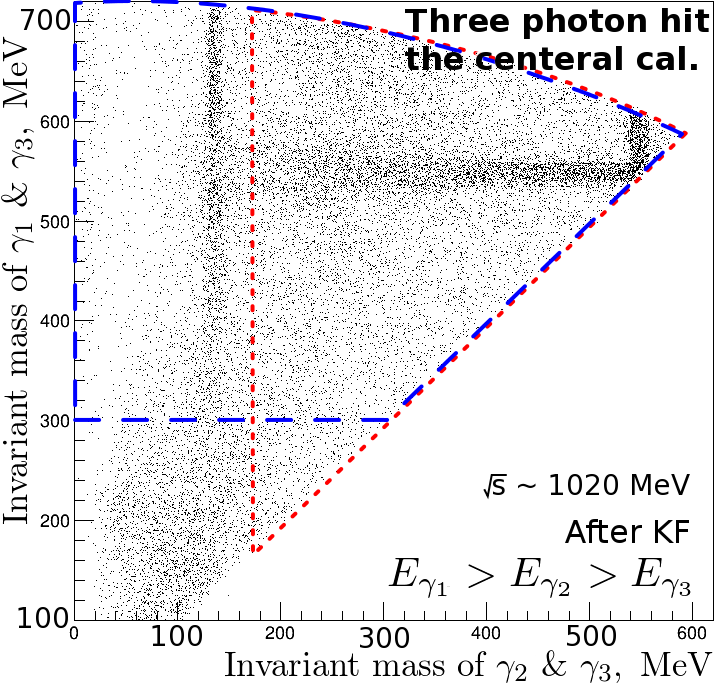
\includegraphics[width=\textwidth]{img/cm12cal2.png}
		\caption{Диаграмма Далица для событий $e^+ e^- \to 3 \gamma$ после кинематической реконструкции,
			когда все три фотона попали в \ce{LXe} калориметр.
			Данные эксперимета, сезон 2013 $\omega \ \phi$, $E_{\text{beam}} = \SI{510}{\MeVr}$.
			Синей линией обозначена кинематическая область используемая для определения числа событий $\pi^0 \gamma$,
			красная линия --- $\eta \gamma$.}
	\end{minipage}
	\hfill
	\begin{minipage}[T]{.48\textwidth}
		\centering
		\label{fig:etag}
		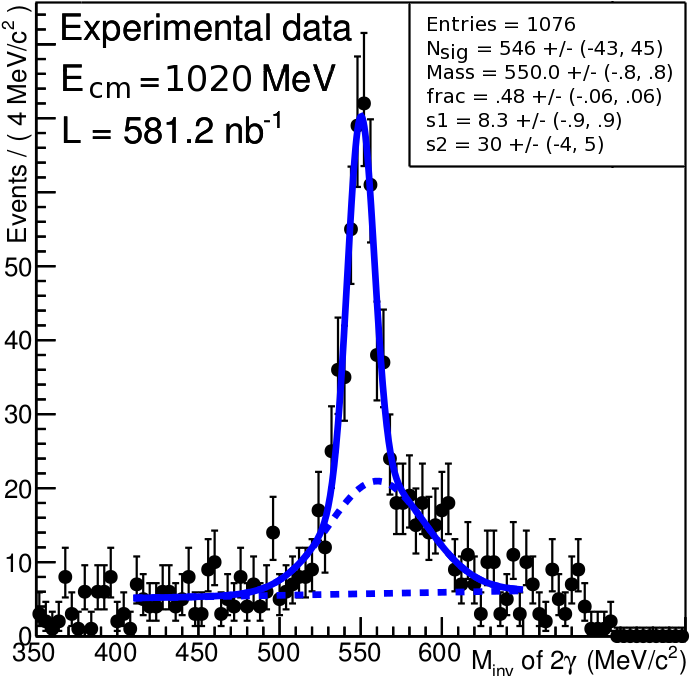
\includegraphics[width=\textwidth]{img/etag.png}
		\caption{Распределение по инвариантной массе двух фотонов после кинематической реконструкции,
			когда все три фотона попали в \ce{LXe} калориметр.
			Данные эксперимета, сезон 2013 $\omega \ \phi$, $E_{\text{beam}} = \SI{510}{\MeVr}$.
			Сплошной синей линией показана аппроксимирующая кривая $f_{\text{sig}} + f_{\text{bkg}}$.
			Синими штрихованами линиями показаны $f_{\text{bkg}}$ и сумма $f_{\text{bkg}}$ и одна составляющая $f_{\text{sig}}$.}
	\end{minipage}
\end{figure}

При построении таких распределений используется ряд дополнительных критериев на параметры частиц их системы в целом.
Минимальное число фотонов зарегистрированных в центральной части калориметра является одним из самых существенных таких отборов.
Для него используется два критерия,
либо хотя бы один фотон летит в цилиндрический калориметр,
либо все фотоны зарегистрированы в цилиндрической части.
Второй набор событий является подклассом первого.
Также второй набор аналогичен отборам проводимым при анализе на детекторе КМД-2,
что делает его более интересным для сравнения результатов.
Данный отбор даёт выбрать в пользу большей статистики или лучшего разрешения по инвариантной массе.

Вторым важным отбором является условие на минимальную энергию фотона,
как правило, она ставится равной \SI{50}{\MeVr}.
Данное число выбрано согласно моделированию и,
с одной стороны, подавляет фон в калориметре,
особенно в его торцевой части, с другой,
оказывает малое влияние на число сигнальных событий.
Таким образом возрастает отношение сигнал/фон.

Существует ещё условие на число зарегистрированных фотонов в событии.
В области $\phi$-мезона,
где сечение $e^+ e^- \to \eta \gamma$ достигает своего максимума,
это позволяет подавить вклад от канала распада $\eta \to \pi^+\pi^-\pi^0$,
ставя ограничение на число фотонов $n < 6$.

Непосредственно для определения числа сигнальных событий проводится подгонка распределения суммой сигнальной и фоновой функций.
Для описания фона используется полином.
Сигнал же описывается суммой нормальных распределений с общим нормировочным множителем.
Используемый алгоритм отбора событий также направлен на подавление фона,
что часто приводит к его малой статистике и трудности определения формы,
особенно под сигнальным пиком.
Для решения данной проблемы используется моделирование,
своё для каждой точки по энергии,
на которое опирается подгоночная функция --- так называемая одновременная подгонка (simultaneous fit).
В областях по энергии, где сечение мало,
и определение как числа событий сигнала,
так и фона затруднено привело к использованию небинированной подгонки,
которая позволяет в таких скользких ситуациях избежать проблем с выбором подходящего бинирования распределения.
Также для малой статистики вопрос, как правило,
идёт о определении верхнего предела, что, как временное решение,
приводит к определению асимметричных ошибок с помощью алгоритма Minos.


\subsection{Определение эффективности отбора}



\subsubsection{Моделирование}

\begin{figure}
	\centering
	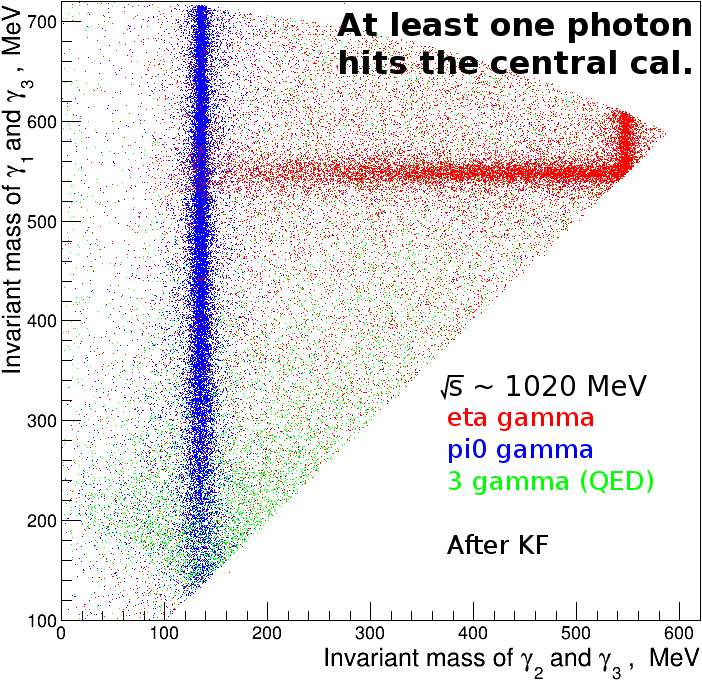
\includegraphics[width=.5\textwidth]{img/cm12mc.png}
	\caption{Диаграмма Далица после КР 
			для событий моделирования в области $\phi$-мезона
			$e^+ e^- \to \pi^0 \gamma$ (синие точки),
			$e^+ e^- \to \eta \gamma$ (красные точки)
			и трёхквантовой аннигиляции (зелёные точки),
			когда хотя бы один фотон попал в \ce{LXe} калориметр.\label{fig:cm12mc}}
\end{figure}

Для определения эффективности отбора событий $e^+ e^- \to \pi^0 \gamma, \, \eta \gamma$ по конченому трёхфотонному состоянию разработанный метод применялся к данным моделирования.
Моделирование проводилось с помощью пакета \emph{GEANT4}, \cite{geant4Allison:2006ve}.
Пример диаграммы Далица приведён на рисунке~\ref{fig:cm12mc}.
В моделирование учитывались все возможные каналы распадов псевдоскалярных мезонов, также моделирование идёт с излучением радиационных фотонов.
% На рисунках \textbf{пара рисунков с эффективностью от с.м. энергии} представлены эффективности при разных условиях отбора в зависимости от полной энергии в системе центра масс.

Падение эффективности с ростом энергии объясняется увеличением вероятности иметь маленькие углы между фотонами в событие,
что приводит к сливанию электромагнитных ливней в калориметре детектора.

Вблизи порога реакции $e^+ e^- \to \eta \gamma$ монохроматичный фотон становится мягким, что уменьшает вероятность регистрации.
Так начиная при энергии системы $\sqrt{s} = \SI{666}{\MeVr}$ энергия монохроматичного фотона равна \SI{30}{\MeVr}, что соответствует порогу на рассмотрения фотона как значащего.

% Для определения эффективности разработанного метода применялся на данных моделирования $e^+ e^- \to
% \eta \gamma$ и $e^+ e^- \to \pi^0 \gamma$.
% Причём с распадом псевдоскалярных мезон во все возможные каналы.
Так характерная эффективность в области $\phi$-мезона без ограничения на углы вылета конечных
фотонов составила \SI{23.7}{\percent} для $\eta \gamma$ процесса.
Для $\pi^0 \gamma$ при условии попадания хотя бы одного фотона в центральную часть детектора
составляет приблизительно \SI{5}{\percent},
при этом наблюдается спад эффективности с ростом $\sqrt{s}$.



\subsubsection{Поправка к эффективности регистрации фотонов}



Эффективность реконструкции фотонов в моделировании и эксперименте определено по событиям процесса
$e^+ e^- \to \pi^+ \pi^- \pi^0 \to \pi^+ \pi^- 2 \gamma$.
Отобранные события разбиваются на два класса:
событие полностью реконструировано и
события с одним потерянным фотоном.


\paragraph{Отбор событий $e^+ e^- \to \pi^+ \pi^- \pi^0$}

На первом этапе отбираются события с двумя центральными треками и с одним или двумя фотонами.
Так же требуется, чтобы флаг is\_bhabha не равнялся 1.
От трека требуется наличие кластера с полярным углом удовлетворяющем условию $0.9 < \theta < \pi - 0.9$.

Для треков определяется отношение энерговыделения к импульсу и
требуется,
чтобы каждое $E_{dep} / p$ лежало в диапазоне $(0.1, \, 2)$.

На каждый фотон накладываются условия:
\begin{itemize}
    \item $| \theta - \pi/2| < 1.4 \approx \ang{80.214}$,
    \item $\SI{15}{\MeVr} < E < 0.75 \sqrt{s}$.
\end{itemize}
После этого должно остаться один или два фотона, чтобы событие осталось в обработке.

Для отобранных частиц вычисляется модуль полного импульса системы $P_{tot}$ и полная энергия $E_{tot}$:
\begin{align}
    E_{tot} &= \sum E_i , \\
    P_{tot} &= \left| \vec{P}_{tot} \right| = \left| \sum \vec{p}_i \right| .
\end{align}
На ни накладываются следующие условия:
\begin{itemize}
    \item $P_{tot} < 0.75 \sqrt{s}$,
    \item $0.25 \sqrt{s} < E_{tot} < 1.75 \sqrt{s}$.
\end{itemize}
\begin{figure}[htbp]
    \centering
    \begin{subfigure}[b]{0.45\textwidth}
        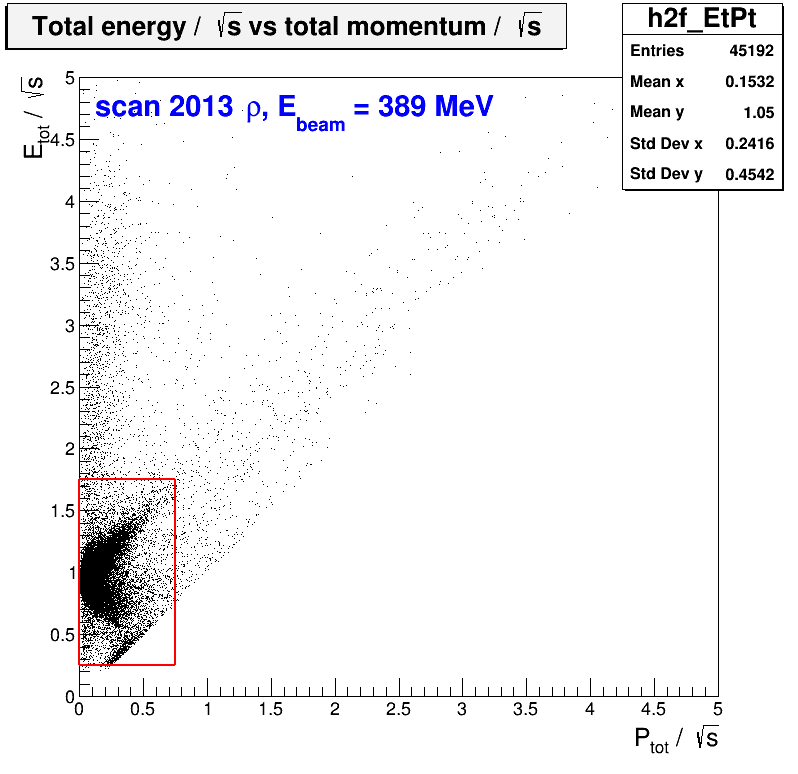
\includegraphics[width=\textwidth]{img/h2f_EtPt.png}
        \caption{Полный вид.}
        \label{fig:EtPt_full}
    \end{subfigure}
    ~
    \begin{subfigure}[b]{0.45\textwidth}
        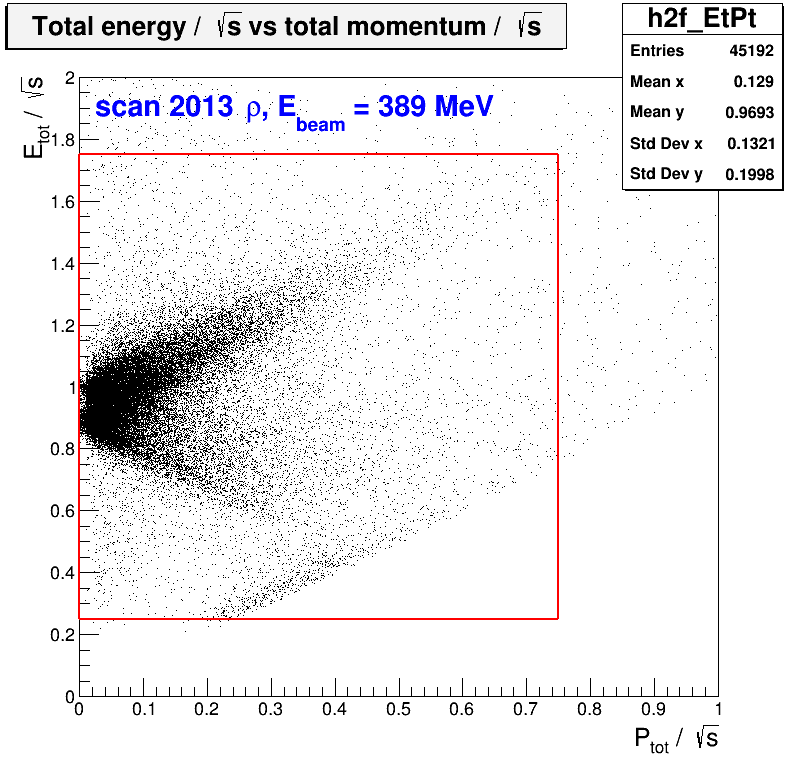
\includegraphics[width=\textwidth]{img/h2f_EtPt_zoom.png}
        \caption{Область выбора приближена.}
        \label{fig:EtPt_zoom}
    \end{subfigure}
    \caption{Распределение полной энергии и полного импульса системы,
        нормированные на $\sqrt{s}$.
        Красной линией обозначены условия отбора.
        Экспериментальные данные сезона $2013 \, \rho$,
        $E_{beam} = \SI{389}{\MeVr}$.}\label{fig:EtPt}
\end{figure}

Для прошедших отборы событий проводится кинематическая реконструкция в гипотезе четырёх частиц (двух заряженных пионов и двух фотонов) с требованием выполнения законов сохранения импульса-энергии для всей системы.
Таким образом после кинематической реконструкции суммарный импульс системы $P^{KF}_{tot}$ стремится к нулю,
а общая энергия системы $E^{KF}_{tot}$ к энергии двух пучков.
\begin{figure}[htbp]
    \centering
    \begin{subfigure}[t]{0.45\textwidth}
        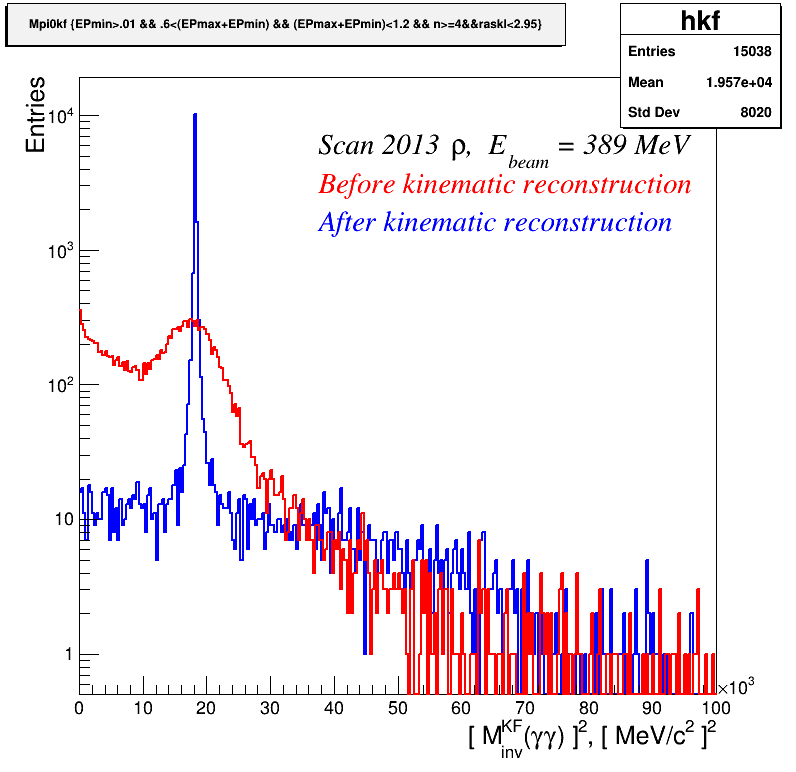
\includegraphics[width=\textwidth]{img/diff_kf_mpi0_2013rho389.png}
        \caption{Данные сезона $2013 \, \rho$, $E_{beam} = \SI{389}{\MeVr}$.}
        \label{fig:diff_kf_mpi0_2013rho389}
    \end{subfigure}
    ~
    \begin{subfigure}[t]{0.45\textwidth}
        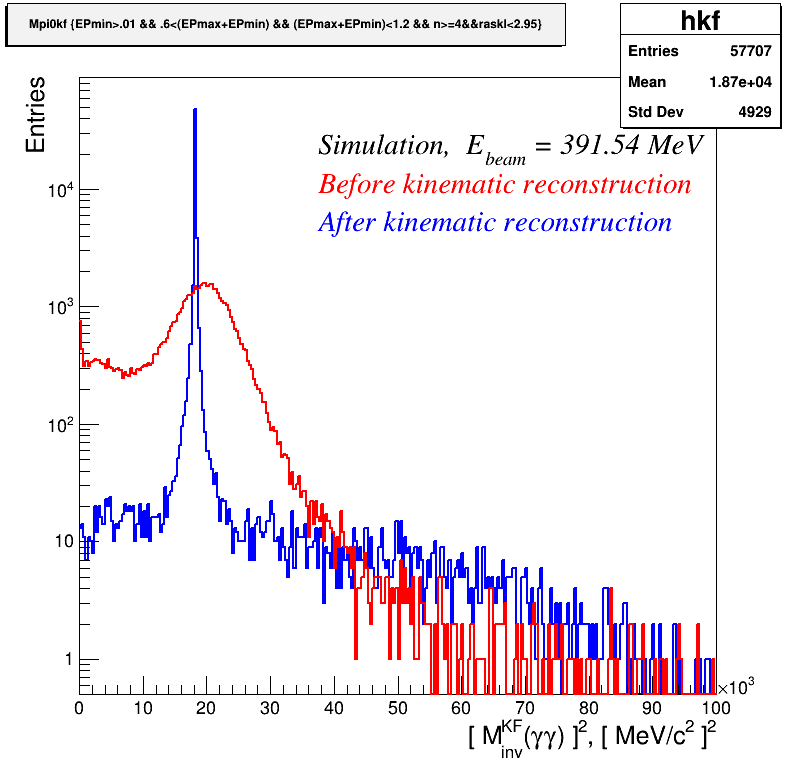
\includegraphics[width=\textwidth]{img/diff_kf_mpi0_sim391_54.png}
        \caption{Моделирование $e^+ e^- \to \pi^+ \pi^- \pi^0$, $E_{beam} = \SI{391.54}{\MeVr}$.}
        \label{fig:diff_kf_mpi0_sim391_54}
    \end{subfigure}
    \caption{Распределение событий по квадрату инвариантной массы двух фотонов для событий с двумя и более фотонами.
    Красная (синяя) гистограмма --- до (после) кинематической реконструкции.}\label{fig:diff_kf_mpi0}
\end{figure}

 
Второй этап отборов начинается с требования на массу отдачи двух заряженных пионов $M_{recoil}^{\pi^+ \pi^-}$,
а именно $\SI{0}{\MeVr} < M_{recoil}^{\pi^+ \pi^-} < \SI{300}{\MeVr}$.
Дополнительно для треков накладывается условие
% $ 0.1 < E_1/p_1 , \, E_2/p_2 < 2 $.
$ E_1/p_1 + E_2 / p_2 < 1$
и $\min(E_i / p_i) > 0.1$.
В то время как на угол между треками $\Omega_{\pi^+ \pi^-}$ накладывается условие $\Omega_{\pi^+ \pi^-} < 2.95$.
Данное условие продемонстрировано на рисунках~\ref{fig:raskl}.
\begin{figure}
    \begin{minipage}[t]{0.45\textwidth}
        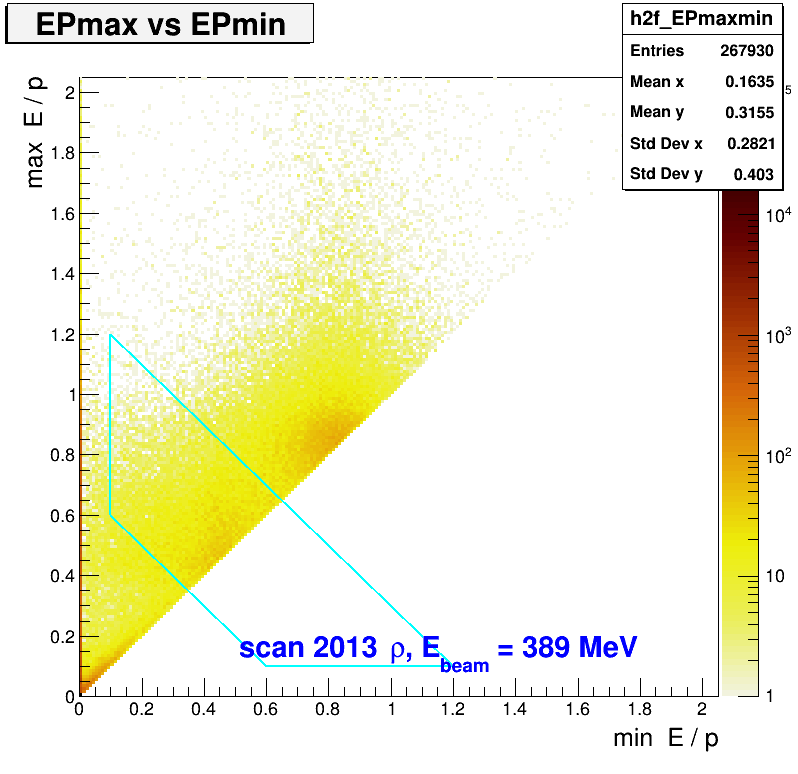
\includegraphics[width=\textwidth]{img/h2f_EPmaxmin_zoom.png}
        \caption{Распределение отношения энерговыделения трека к импульсу трека.
            Голубой линией обозначены условия отбора по $E_i / p_i$.
            Экспериментальные данные сезона $2013 \, \rho$, $E_{beam} = \SI{394}{\MeVr}$.}
        \label{fig:EPmaxmin_zoom}
    \end{minipage}
    \qquad
    \begin{minipage}[t]{0.45\textwidth}
        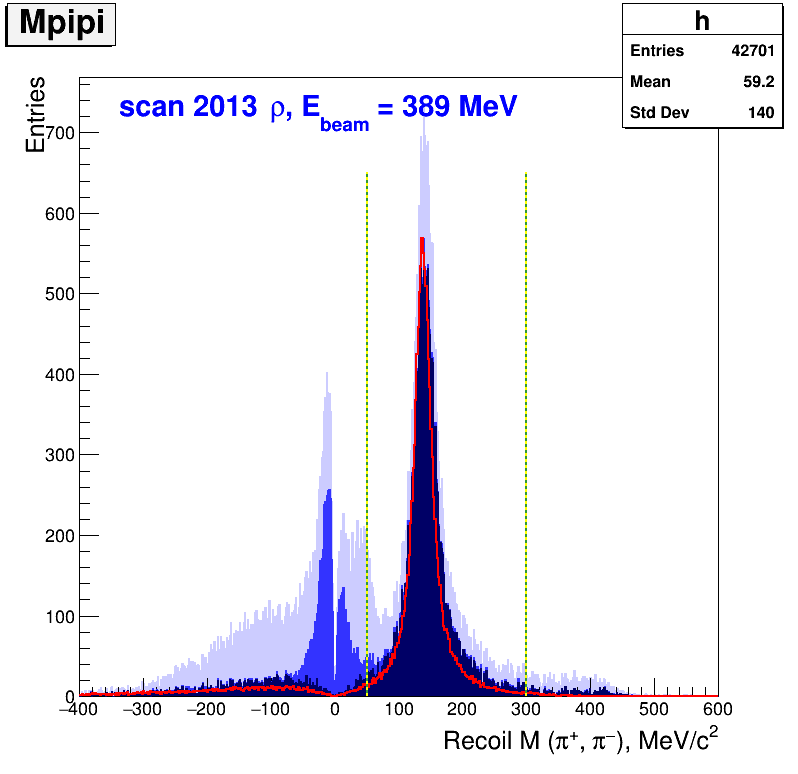
\includegraphics[width=\textwidth]{img/mpipi.png}
        \caption{Тёмно-синяя гистограмма --- с отбором по $E/p$ и $\Omega_{\pi^+ \pi^-}$,
            синяя гистограмма --- с отбором по $E/p$,
            блеклая гистограмма --- до отбора по $E/p$,
            красная линия --- моделирование после отбора по $E/p$ и $\Omega_{\pi^+ \pi^-}$,
            зелёно-жёлтая штрихованная линии --- условия отбора по $M_{recoil}^{\pi^+ \pi^-}$.}
        \label{fig:mpipi}
  \end{minipage}
\end{figure}


\begin{figure}[htbp]
    \centering
    \begin{subfigure}[b]{0.45\textwidth}
        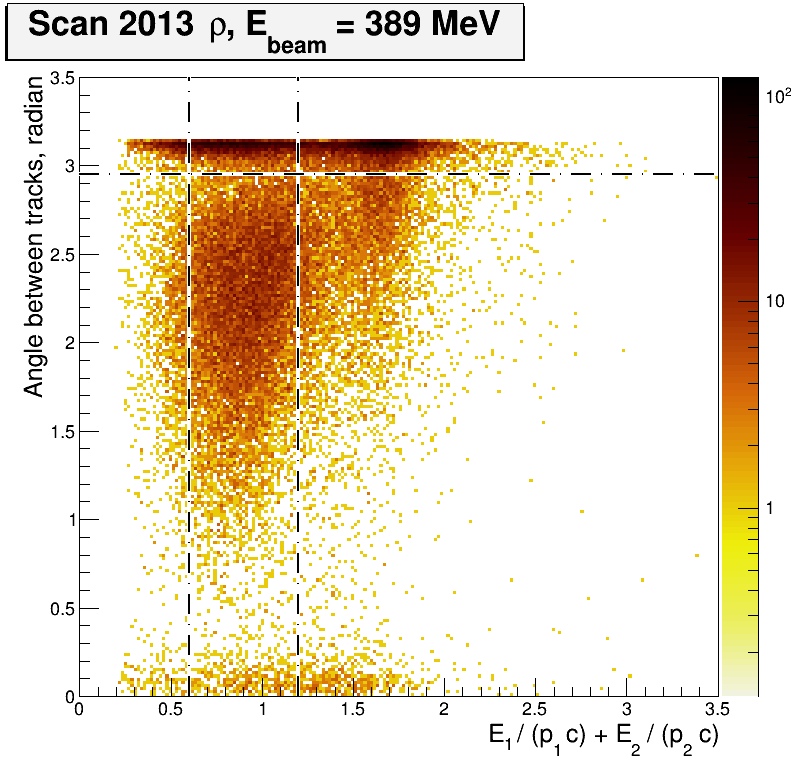
\includegraphics[width=\textwidth]{img/raskl_vs_sumEP_rho389.png}
        \caption{Данные сезона $2013 \, \rho$, $E_{beam} = \SI{389}{\MeVr}$.}
        \label{fig:raskl_rho389}
    \end{subfigure}
    ~
    \begin{subfigure}[b]{0.45\textwidth}
        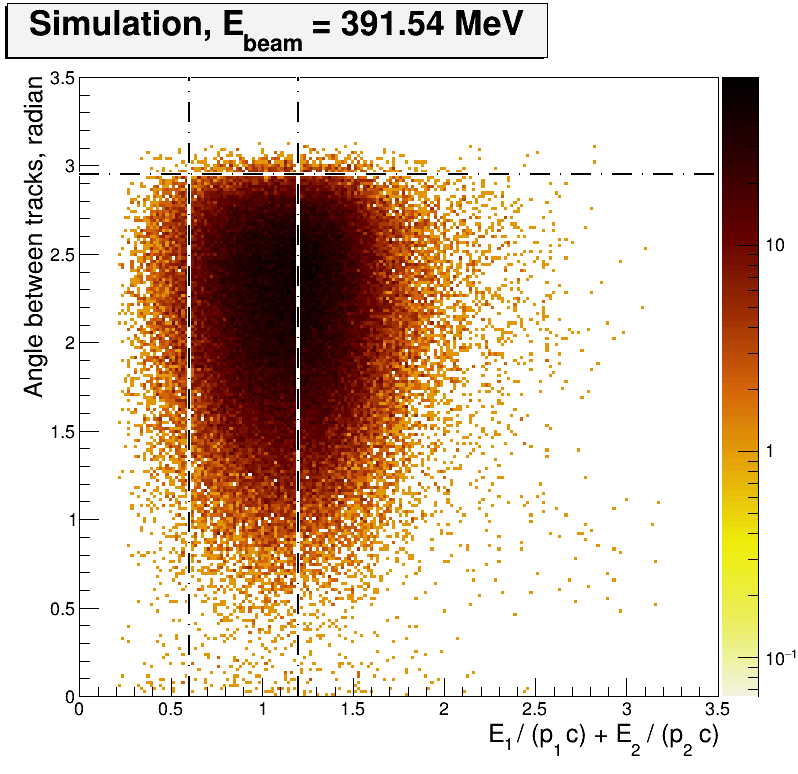
\includegraphics[width=\textwidth]{img/raskl_vs_sumEP_sim391_54.png}
        \caption{Simulation $\pi^+ \pi^- \pi^0$, $E_{beam} = \SI{391.54}{\MeVr}$.}
        \label{fig:raskl_sim391_54}
    \end{subfigure}
    \caption{Distribution of an angle between tracks $\Omega_{\pi^+ \pi^-}$ versus $E_1/p_1 + E_2 / p_2 < 1$.
    Vertical lines represent the used cut on $\sum E_i / p_i$.}\label{fig:raskl}
\end{figure}




\subsubsection{Эффективность триггера}

Вычисление сечений изучаемых реакций требует учёта эффективности нейтрального триггера $\varepsilon_{NT}$,
которая извлекается по событиям радиационного баба рассеяния $e^+e^- \to e^+e^-\gamma$.


Процесс $e^+e^- \to e^+e^-\gamma$ выбран по ряду причин.
Он похож по характеру энерговыделения,
так как и фотоны,
и электроны рождают электромагнитный ливни.
Количество частиц в конечном состоянии равно оному в изучаемых процессах,
а именно трём.
Из первых двух пунктов следует,
что и система нейтрального триггера будет реагировать похожим образом
---
срабатывают те же маски.
В процессе есть как заряженные,
так и нейтральная частицы,
что позволяет использовать две независимые подсистемы запуска детектора,
позволяющие изучать вероятность срабатывания друг друга.
% что позволяет использовать особенности триггера детектора КМД-3
% ---
% две независимых подсистемы запуска детектора.
Сечение процесса $e^+e^- \to e^+e^-\gamma$ плавное и достаточно велико во всей доступной области энергий.


Отбираются события с двумя центральными треками и хотя бы одним фотоном,
при этом на гамма-кванты налагаются дополнительные условия, 
как $0.42 < \theta < \pi - 0.42$, 
так и $E_\gamma > \SI{30}{\MeVr}$.
Центральным треком
---
треком лежащим в том числе в области взаимодействия пучков или рядом с ней
---
считается такой трек,
который удовлетворяет следующим условиям:
\begin{itemize}
	\item максимально расстояние между треком и орбитой пучков не более \SI{6}{\cmr} в плоскоти $\rho-\varphi$;
	\item $\chi^2_{R} < 100$ из подгонки хитов ДК в $\rho$--$\varphi$ плоскости;
	\item $\chi^2_{Z} < 100$ из подгонки хитов ДК в $\rho$--$z$ плоскости.
\end{itemize}
Более того требуется, чтобы хотя бы одна из частиц летела в цилиндрический калориметр:
$ 0.9 < \theta < \pi - 0.9 $.
Последние условие,
как правило,
обеспечивается одним из треков,
ввиду неэффективности восстановления треков при малых полярных углах.

Затем для каждого события вычисляется полная энергия $E_{sys}$ и полный импульс $P_{sys}$ системы частиц,
причём для нейтральных частиц импульс приравнивается к их энергии, а энергия заряженных частиц рассчитывается как $E = \sqrt{p^2 + {m_e}^2}$.
Таким образом последние частицы предполагаются электронами или позитронами с массой $m_e$.
На полный импульс $P_{sys}$ и полную энергию $E_{sys}$ полученной системы частиц накладываются нижеприведённые условия:
\begin{itemize}
    \item $P_{sys} < 0.25 \sqrt{s}$;
    \item $\frac{2}{3} \sqrt{s} + P_{sys} < E_{sys} < 1.25 \sqrt{s}$.
\end{itemize}
Для определения эффективности триггера отбираются события с $\min (E/p) > 0.8$ и $\max (E/p) < 2$.
Такое условие позволяет дополнительно подавить
фон от минимально ионизирующих частиц $\pi^\pm$ и $\mu^\pm$.
при этом происходят два вида отборов с количеством летящих в цилиндрическую часть детектора частиц:
не меньшим одного и не меньше трёх.


Дополнительно для каждого события сохраняется информация о том,
какой из триггеров сработал:
\begin{itemize}
  \item нейтральный триггер;
  \item заряженный триггер;
  \item полный триггер, то есть в событие сработал и заряженный, и нейтральный триггер.
\end{itemize}
Теперь для каждой точки по энергии определяются количества событий, в которых сработал:
\begin{itemize}
  \item только нейтральный триггер --- $N_{NT}$;
  \item только заряженный триггер ---  $N_{CT}$;
  \item полный триггер --- $N_{tot}$.
\end{itemize}
На основе этих данных рассчитывается эффективности нейтрального триггера $\varepsilon_{NT}$,
заряженного триггера $\varepsilon_{CT}$ и полного триггера $\varepsilon_{tot}$.
Пусть произошло $N$ событий $e^+ e^- \to e^+ e^- \gamma$,
тогда можно записать систему уравнений:
\begin{align}
    N_{NT} &= \varepsilon_{NT} \cdot ( 1 - \varepsilon_{CT} ) \cdot N , \\
    N_{CT} &= ( 1 - \varepsilon_{NT} ) \cdot \varepsilon_{CT} \cdot N , \\
    N_{NT} &= \varepsilon_{NT} \cdot \varepsilon_{CT} \cdot N .
\end{align}
Разрешим данные связи относительно искомых эффективностей:
\begin{align}
    \varepsilon_{NT} &= \frac{ N_{tot} }{ N_{tot}+N_{CT} } , \\
    \varepsilon_{CT} &= \frac{ N_{tot} }{ N_{tot}+N_{NT} } , \\
    \varepsilon_{tot} &= 
    \frac{ N_{tot} (N_{tot}+N_{CT}+N_{NT}) }{
        (N_{tot}+N_{CT}) (N_{tot}+N_{NT})
    } \\
    &=
    1 - (1-\varepsilon_{NT}) (1-\varepsilon_{CT}) .
\end{align}
Положив статистическую неопределённость $N_i$,
где $i = NT, \, CT,$ и $tot$,
равными $ \Delta N_i  = \sqrt{N_i} $ можно вычислить погрешности определения эффективностей,
воспользовавшись формулой переноса ошибок.
\[ \Delta  \varepsilon_{NT} = \frac{1}{ ( N_{TC} + N_T )^2} \left[ N_{TC}  N_T ( N_{TC} + N_T )
\right]^\frac{1}{2} \]
\[ \Delta  \varepsilon_{CT} = \frac{1}{ ( N_{TC} + N_C )^2} \left[ N_{TC}  N_C ( N_{TC} + N_C )
\right]^\frac{1}{2} \]
\[ \Delta  \varepsilon_{tot} =  \left[ (1-\varepsilon_{NT})^2 {\Delta  \varepsilon_{CT}}^2 +
(1-\varepsilon_{CT})^2 {\Delta  \varepsilon_{NT}}^2 \right]^\frac{1}{2} \]

Основными фоновыми процессам для $e^+ e^- \to e^+ e^-\gamma$ являются процессы
$e^+ e^- \to \pi^+ \pi^- \gamma$ и $e^+ e^- \to \pi^+ \pi^- \pi^0 \to \pi^+ \pi^- 2\gamma$.
Так как эти процессы носят резонансный характер,
то их вклад в ошибку определения эффективности триггера будет наиболее большим в области $\omega (782)$ и $\phi (1020)$ резонансов.
Для подавление событий с заряженными пионами используется ограничение на отношение импульса частицы,
измеренного трековой системой детектора, к энергии, определённой по данным калориметра.
Для электронов и позитронов это отношение близко к единице.
В случае пионов оно пикуются в области $P/E = \sqrt{1 - {m_{\pi^\pm}}^2 / E^2}$,
так для энергии пиона равной \SI{300}{\MeVr} расчётное $P/E \simeq 0.88$.

Далее определялась эффективность нейтрального триггера,
а также заряженного и полного, в зависимости от диапазона полярных углов частиц.
Будем накладывать ограничение на минимальный угол $\theta_{min}$ между частицами и осью пучков.
Из рисунка \textbf{рисунок} видно,
что начиная с $\theta_{\min} = 0.9$ эффективность стабилизируется и перестаёт зависеть от $\theta_{\min}$,
далее для определения эффективности триггера будет использоваться именно это значение минимального угла.

Теперь определим эффективности триггеров для всей статистики, используемой в данной работе.
На рисунке~\ref{fig:nt_eff} представленность зависимость эффективностей от энергии в системе центра масс.
Видно, что области резонансов наблюдаются некоторые провалы в эффективностях,
наиболее ярко это видно для заряженного триггера.


\begin{figure}
    \centering
    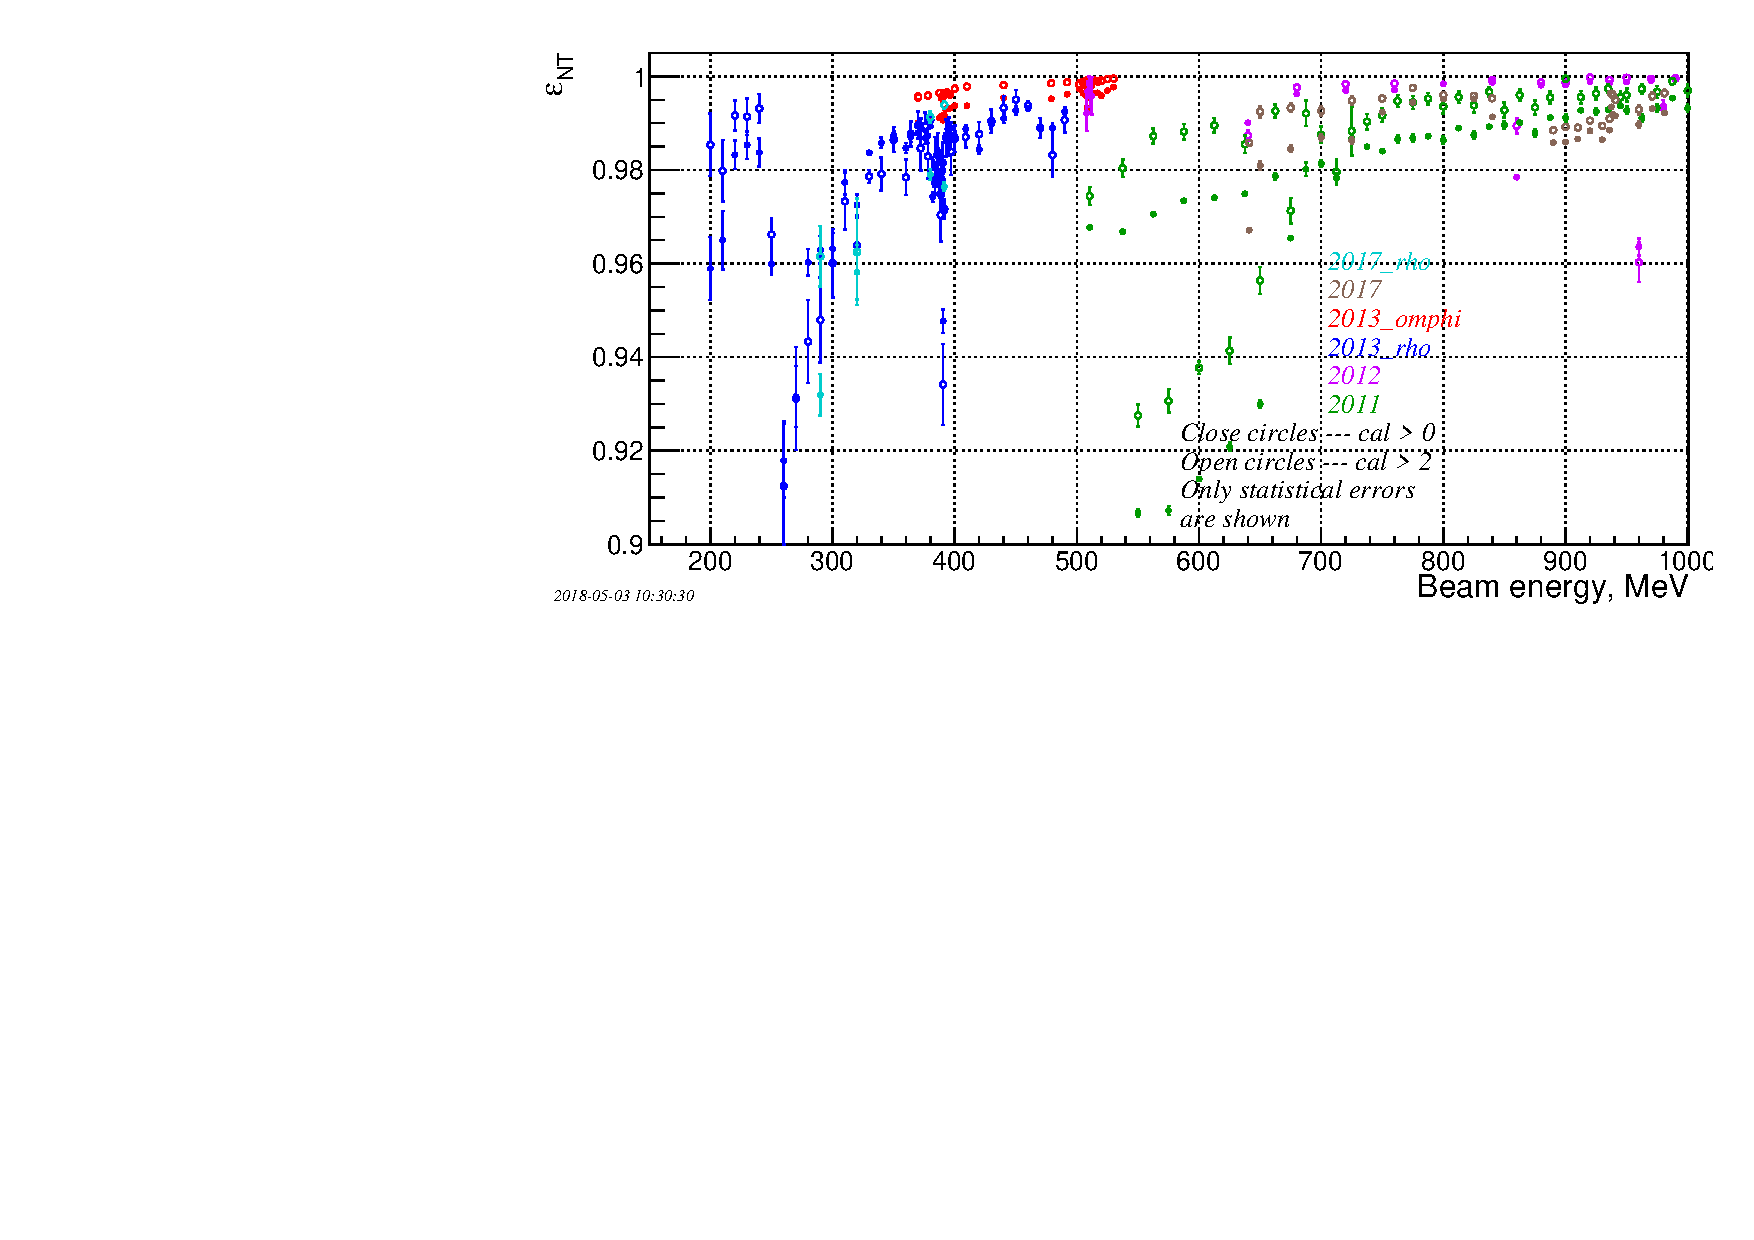
\includegraphics[width=\textwidth]{img/nt_eff.pdf}
    \caption{Эффективность нейтрального триггера.}
    \label{fig:nt_eff}
\end{figure}



% \subsubsection{Учёт радиационных поправок}


\subsection{Сечение процессов}

Основной задачей данной работы является вычисление сечение реакций
$e^+e^- \to \pi^0 \gamma, \, \eta \gamma$ в доступном диапозоне энергий.
Сечение расчитывается согласно формуле
\begin{equation}
	\sigma = \frac{ N } { L \, (1+\delta_{rad}) \, \varepsilon_{NT} \,
	\varepsilon_{det}} \cdot  
	\left( \frac{ {\varepsilon^{MC}_{\gamma}} }{ {\varepsilon^{exp}_{\gamma}} } \right)^3.
\end{equation}
Здесь $L$ --- интегральная светимость;
$\varepsilon_{det}$ --- эффективность метода, определяется из моделирования;
$\delta_{rad}$ --- радиационная поправка;
$\varepsilon_{NT}$ --- эффективность нейтрального триггера;
вторая дробь соответствует поправке на разницу между моделированием и экспериментом в эффективности
реконструкции фотонов.

Радиационная поправка $\delta_{rad}$ считается по алгоритму, основанному на статье \cite{Kuraev1985}.
Данная поправка является радиационной поправкой к процессам однофотонной аннигиляции $e^+ e^-$-пары,
связанная только с начальным состоянием.
Заявленная точность вычислений не хуже \SI{0.1}{\percent}.
В такую же точность оценивается и вычисление радиационной поправки,
главным образом определяемая алгоритмом аппроксимации сечений интересуемого процесса.
Вычисленные значения $1+\delta_{\text{rad}}$ приведены на рисунке~\ref{fig:rad_corr}.

\begin{figure}[htbp]
	\centering
	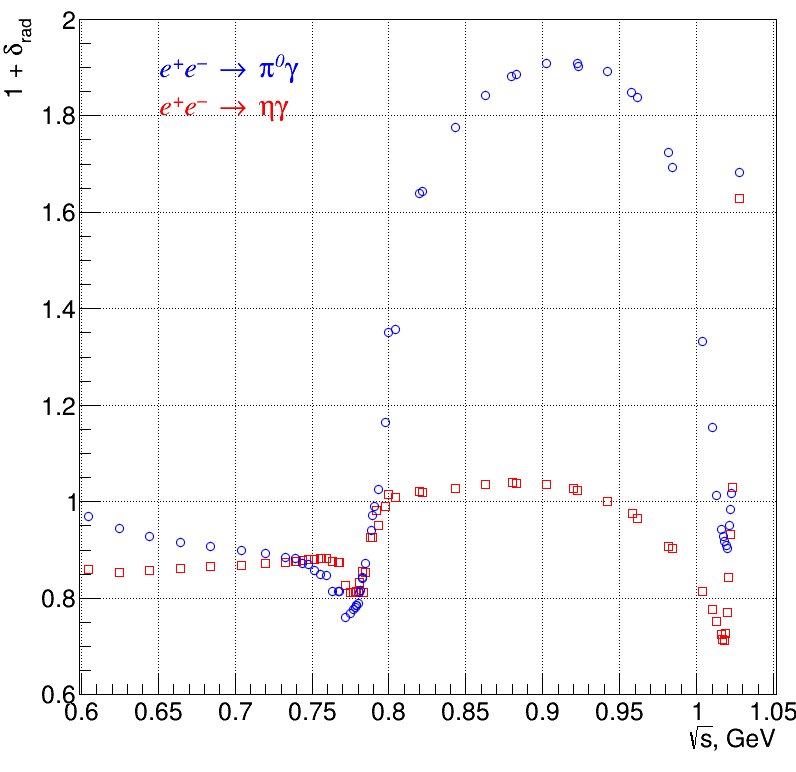
\includegraphics[width=.5\textwidth]{img/rad_corr_for_pseudodisser.png}
	\caption{Радиационная поправка $1+\delta_{\text{rad}}$ для процессов
		$e^+ e^- \to \pi^0 \gamma$ (синие кружки),
		и $e^+ e^- \to \eta \gamma$ (красные квадраты).}\label{fig:rad_corr}
\end{figure}

Инетгральная светимость $L$ на детекторе КМД-3 определяется по процессу Баба рассеяния
$e^+e^- \to e^+e^-$ на большой угол $0.9 < \theta < \pi - 0.9$,
\cite{Ryzhenenkov:2017xqu}.
Достоверность полученных значений контролируется по результатам интгрального сечения $L_{\gamma \gamma}$,
извлекаемого из процесса $e^+e^- \to \gamma \gamma$,
также рассматриваемого в больших углах.
Отличие $1 - L / L_{\gamma \gamma}$ от 0 менее \SI{1}{\percent},
здесь точность ограничено статистикой $e^+e^- \to \gamma \gamma$.

Предварительные результаты по сечения реакций представлены в на рисунках~\ref{fig:cs_pi0g_mine} и~\ref{fig:cs_etag_mine}.

\begin{figure}[htbp]
	\begin{minipage}[T]{.48\textwidth}
		\centering
		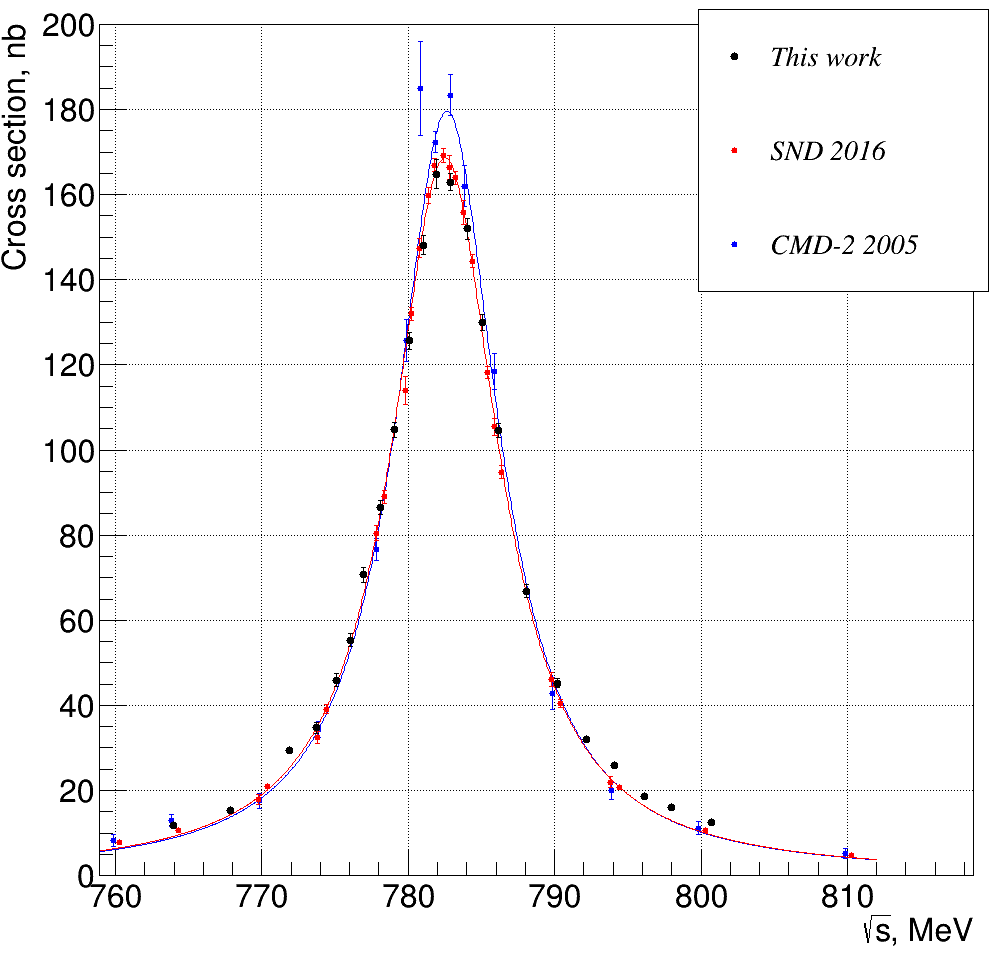
\includegraphics[width=\textwidth]{img/my_pi0g_cross_section_for_pseudodisser.png}
		\caption{Сечение $e^+ e^- \to \pi^0 \gamma$:
			чёрные точки --- предвариетльные результаты данной работы,
			красные (синие) точки и линия --- результаты \cite{Achasov:2016bfr} (\cite{Akhmetshin:2004gw})
			и их аппроксимация нерелятивистк функцией Брейта--Вигнера.}\label{fig:cs_pi0g_mine}
	\end{minipage}
	\begin{minipage}[T]{.48\textwidth}
		\centering
		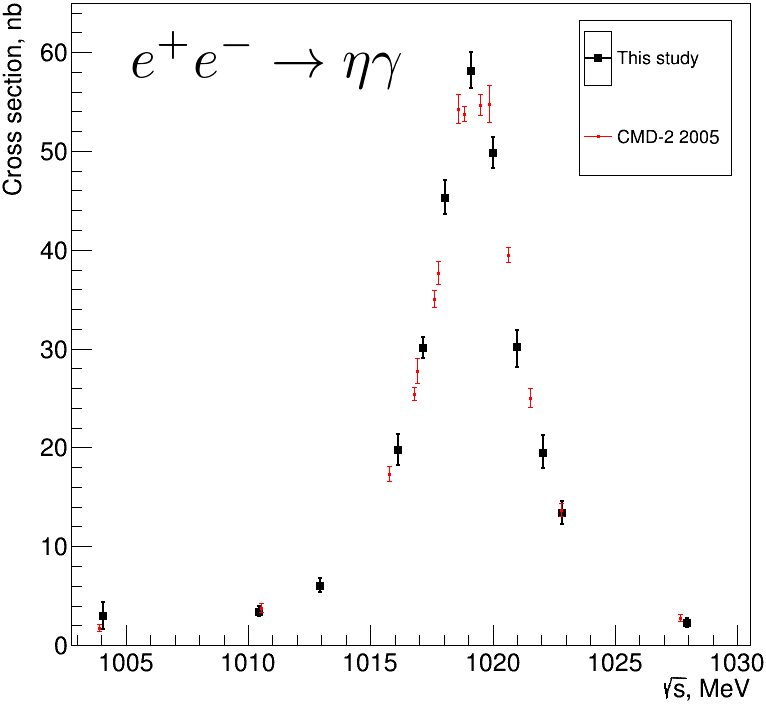
\includegraphics[width=\textwidth]{img/cs_etag_at_phi.png}
		\caption{Сечение $e^+ e^- \to \eta \gamma$:
			чёрные точки --- предвариетльные результаты данной работы,
			красные точки --- результаты \cite{Akhmetshin:2004gw}.}\label{fig:cs_etag_mine}
	\end{minipage}
\end{figure}

%и $e^+e^- \to \gamma \gamma$.%, \cite{lumAkhmetshin2012b}.
%Такой подход позволяет лучше понять и оценить систематические ошибки, которое находятся на уровне \SI{\sim2}{\percent}.
%В ходе определения светимости используются данные моделирования,
%полученные с помощью Монте-Карло генератора фотонных струй (Monte-Carlo Generator Photon Jets)%, \cite{Arbuzov2006}, \cite{Actis2010}),
%модефицированного для изучения продуктов реакций  $e^+e^- \to e^+e^-, \gamma \gamma$.
%Точность расчёта этих сечений с учётом радиационных поправок лучше, чем \SI{0.2}{\percent}.

%Для сравнения полученных сечений с мировыми данными исользованны результаты работ ... .
%Так как данные для процесса $e^+ e^- \to \eta \gamma$ приведенны для различных мод распада $\eta$-мезона,
%то для перевода сечений к одной шкале используются данные %\cite{Beringer:1900zz}.

% \subsubsection{Аппроксимация сечения}